\documentclass[../../ClassicThesis.tex]{subfiles}
\begin{document}

\section{Platener Is Implemented In {\convertify}}
\label{sec:application-platener}

 % - Section overview
 % - Application is built with Convertify (integration with lifecycle events
 %   and rendering engine)
 % - needs-figure :: Application is separated into Packages
 % - Plugins provide scene feature
 % - Client Code to integrate plugins, system and user interfaces

{\platener} is a web-application that converts 3D-printable
models into laser-cuttable equivalents. This section
describes the implementation of {\platener} within the
{\convertify} framework. Therefore, {\platener} integrates
with the system events and rendering engine of
{\convertify}. As proposed in the preceding section, it uses
several plugins to bring its features to the WebGL
scene. Section~\ref{sec:platener-uses-plugins} describes
these plugins briefly.
Section~\ref{sec:platener-pipeline-plugin} shows
architectural details to the most important plugin:
the \name{PlatenerPipeline} plugin. This plugin
implements different conversion strategies for
{\threedmodel}s. In Section~\ref{sec:client-to-application}
we explain how the application combines user interfaces with
the \class{Dispatcher} and the plugins.

\subsection{Platener Uses Plugins to Implement Its Features}
\label{sec:platener-uses-plugins}

The plugins composed into {\platener} provide its computation
logic and WebgGL scene rendering. We will give a brief introduction of
each plugin in the following paragraphs.
Figure~\ref{fig:plugin-constellation} shows all available plugins of
{\platener}.

\subsubsection{Platener Pipeline Plugin}

The \name{PlatenerPipeline} plugin does the major work on
converting {\threedmodel}s to 2D~plates. The plugin defines
multiple conversion approaches. A conversion is an
approximation of the original model with plates.
Figure~\ref{fig:conversion:plate} and
Figure~\ref{fig:conversion:stacked} show two conversion
results. This plugin generates a set of 2D~paths, so that
the conversion can be produced with a {\lasercutter}. The
paths are depicted in Figure~\ref{fig:conversion:paths}.
Section~\ref{sec:platener-pipeline-plugin} explains the
architecture of the \name{PlatenerPipeline} plugin in
detail.

\begin{figure}[h]
  \centering
  \begin{subfigure}[a]{0.3222\textwidth}
    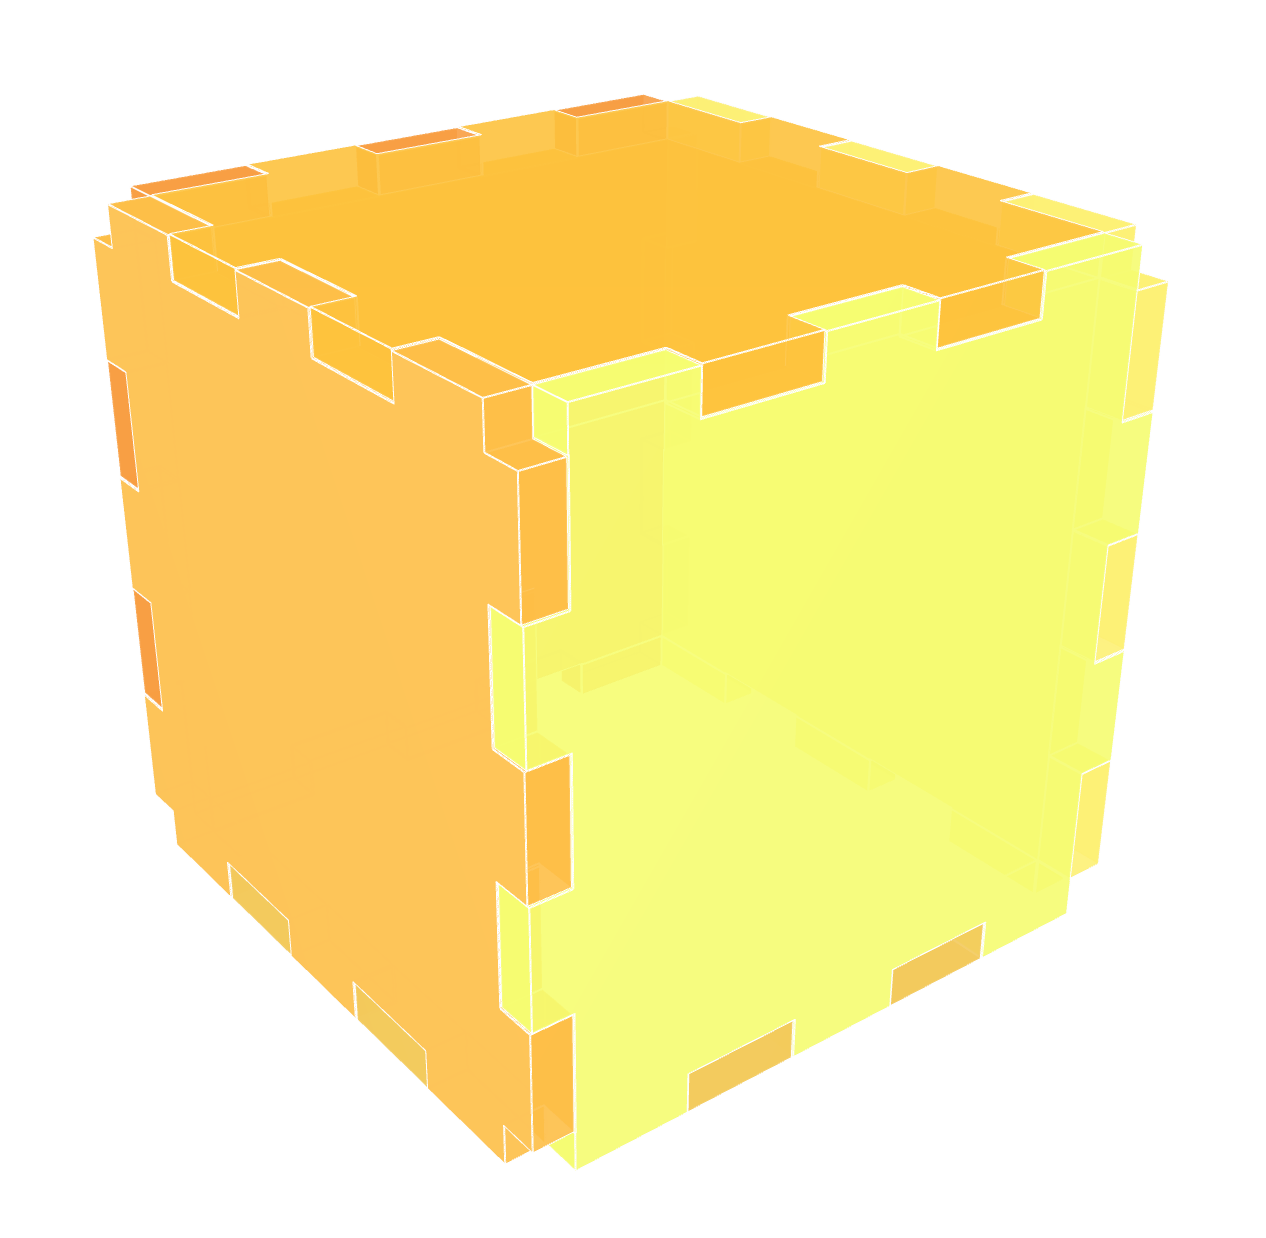
\includegraphics[width=\textwidth]{03-architecture-box-hull}
    \caption{A box converted with hull approximation.}
    \label{fig:conversion:plate}
  \end{subfigure}
  \begin{subfigure}[b]{0.3222\textwidth}
    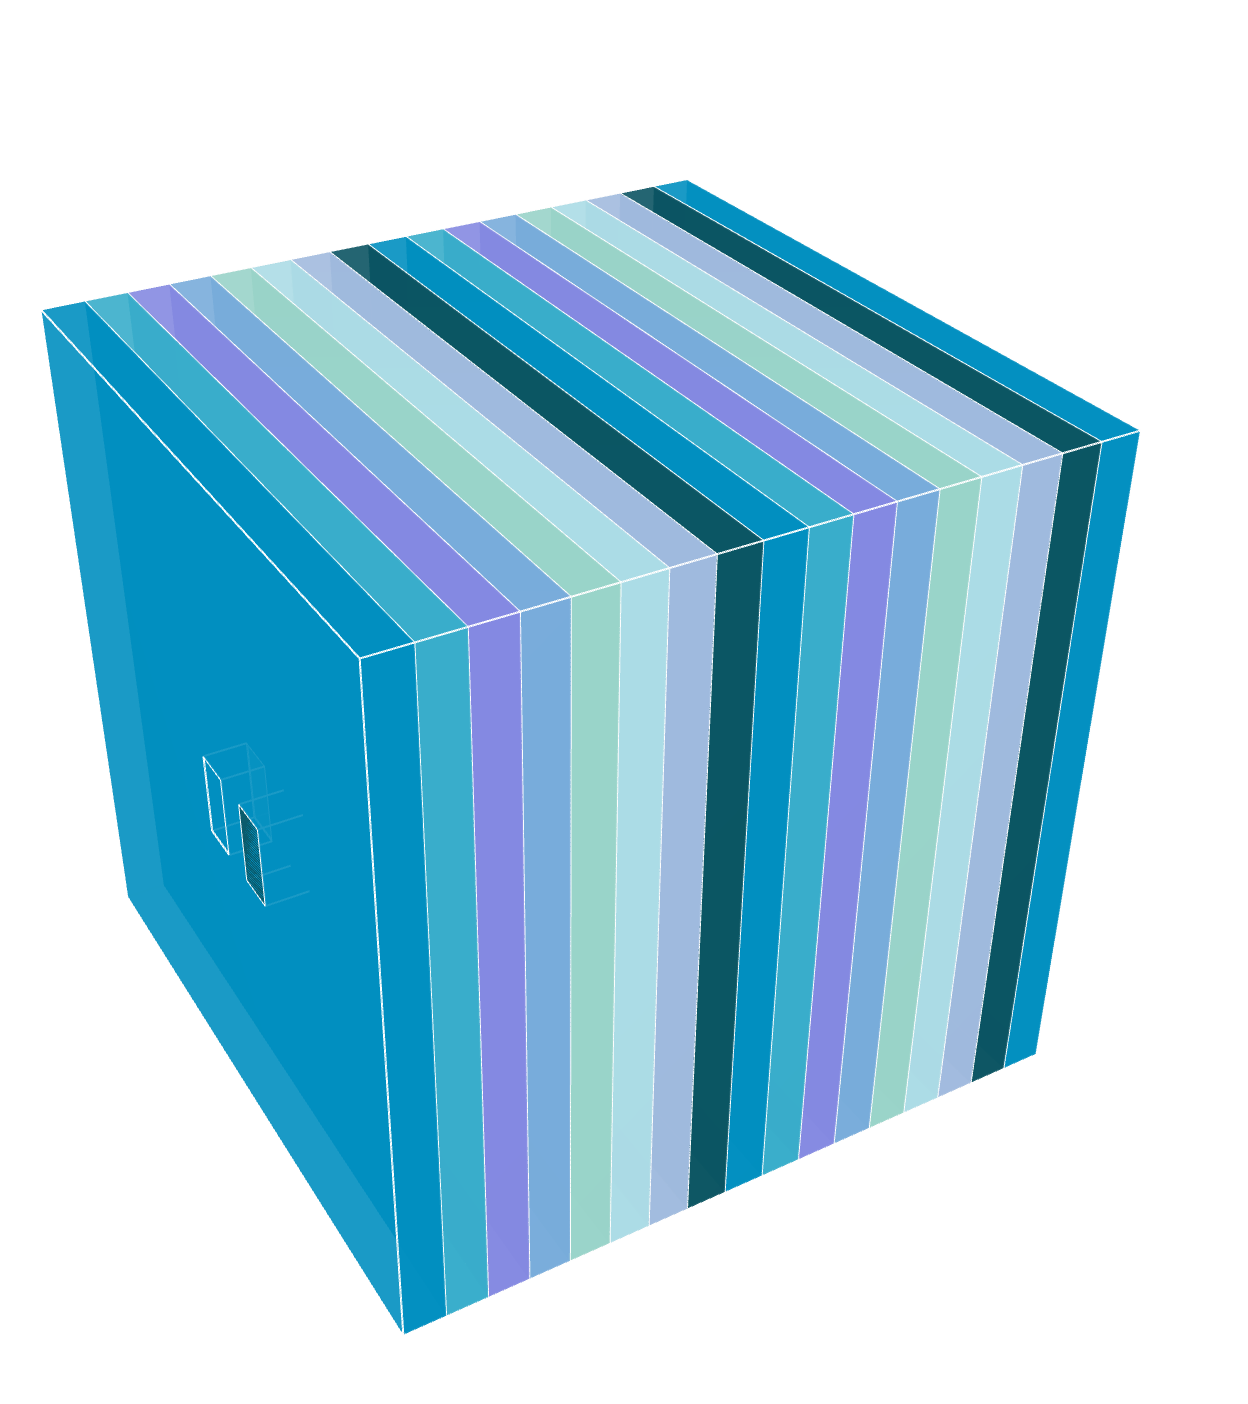
\includegraphics[width=\textwidth]{03-architecture-box-stacked}
    \caption{A box converted with stacked approximation.}
    \label{fig:conversion:stacked}
  \end{subfigure}
  \begin{subfigure}[c]{0.3222\textwidth}
    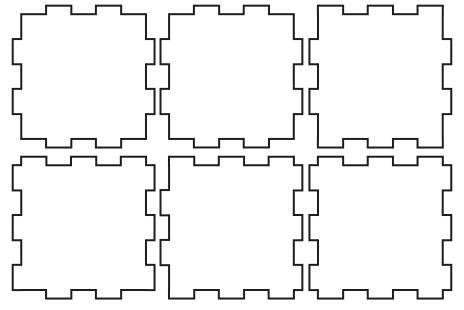
\includegraphics[width=\textwidth]{03-architecture-cutting-plan-box-hull}
    \caption{2D~paths of the box converted with hull approximation.}
    \label{fig:conversion:paths}
  \end{subfigure}
  \caption{Results of the \name{PlatenerPipeline} plugin.}
  \label{fig:conversion}
\end{figure}

% The \name{PlatenerPipeline} plugin is the main computation unit.
% The plugin defines multiple {\fabmethod}s. A
% {\fabmethod} is a conversion approach of a \threedmodel.
% Multiple computation steps, which can manipulate the input
% model, are chained after another to produce 2D- or
% 3D-output. For example, construction plans in the format of
% {\svgfile}s are such an output, see Figure~\ref{}
% \note{construction plans figure}.
% Section~\ref{sec:platener-pipeline-plugin} explains the
% architecture of the \name{PlatenerPipeline} plugin in detail.

\subsubsection{Node Visualizer Plugin}

We visualize the results of the \name{PlatenerPipeline}
plugin in the WebGL view. The \name{NodeVisualizer} plugin
renders the results of each conversion and its intermediate
computation steps respectively. With the help of this we
debug the results of the computation visually. As explained
in Section~\ref{ch:userinteraction}, we select a
single visualization at a time to inspect the results of the
step associated with the visualization.
Figure~\ref{fig:steps-plate} shows a head-mounted display in
the \name{Plate} step.
% Figure~\ref{fig:steps:ui} shows the
% selection of that visualization in the user interface.

\begin{figure}[h]
  \centering
  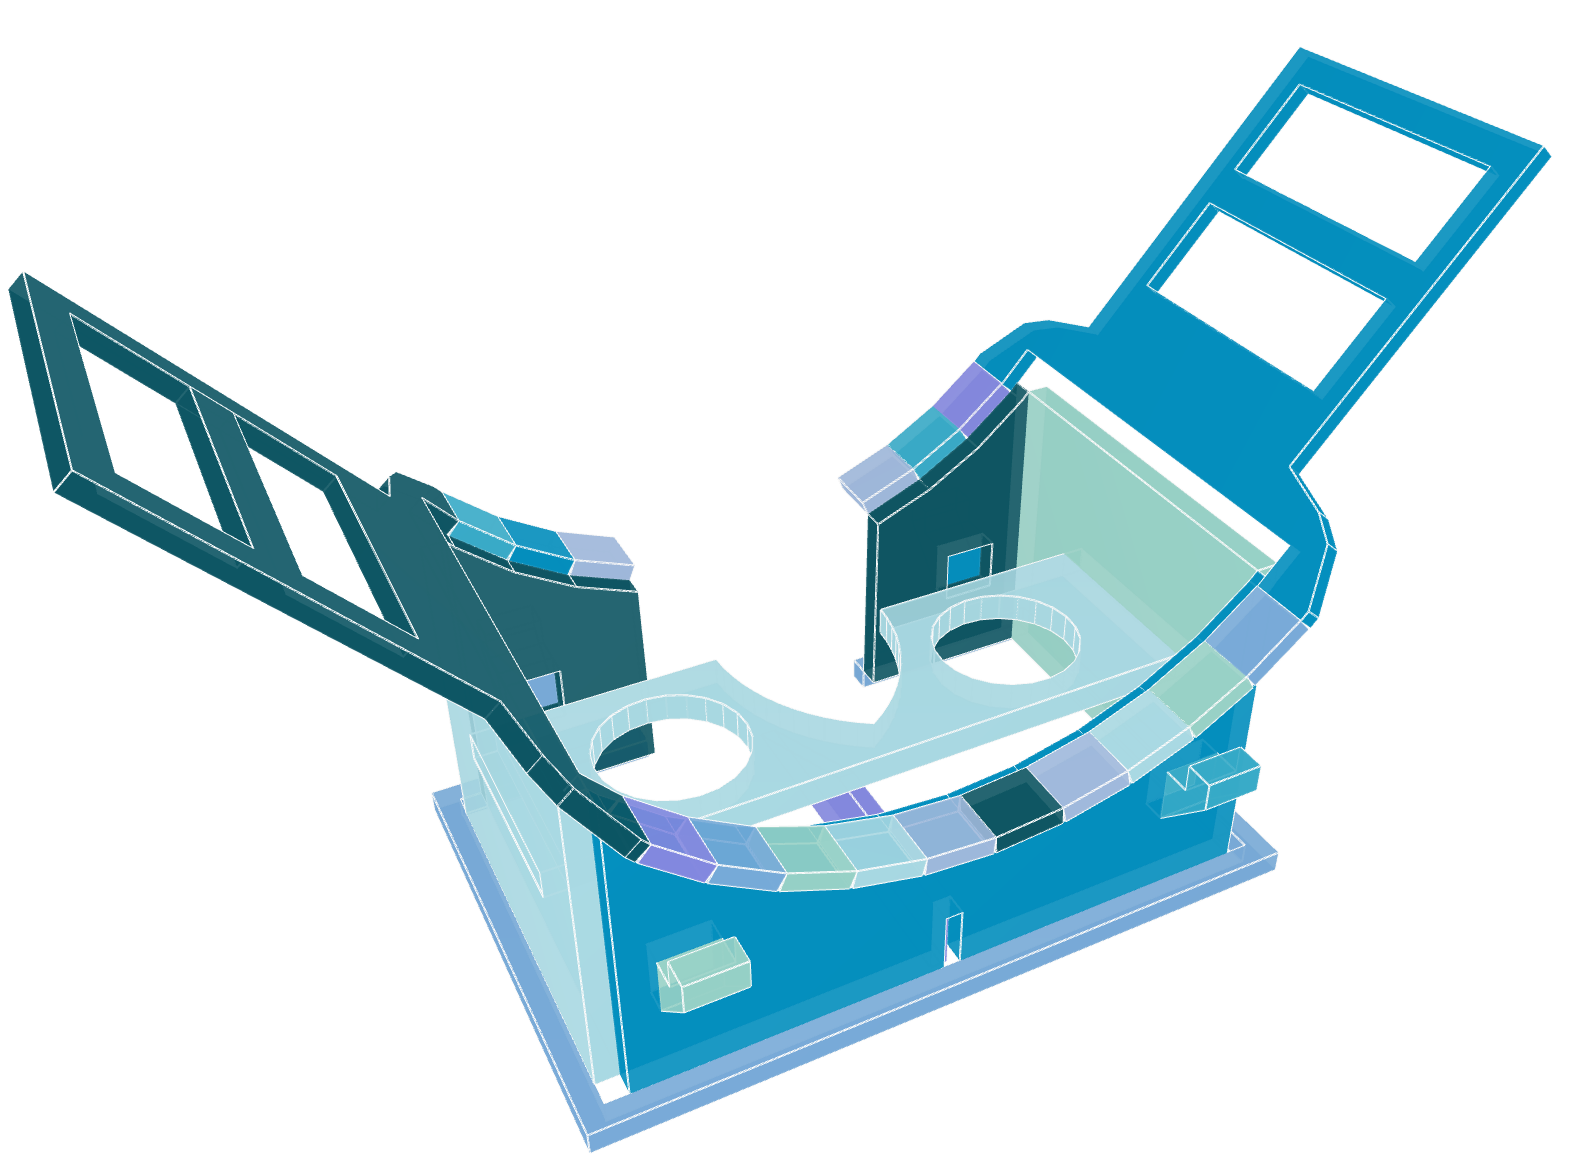
\includegraphics[width=\textwidth]{03-architecture-hmd-plates}
  \label{fig:steps-plate}
  \caption{Visual debugging of intermediate conversion
    results.A head-mounted display, consisting of plates
    only.}
\end{figure}

\subsubsection{Scorer Plugin}

We run multiple conversion approaches sequentially and choose
the best fitted conversion as output. Therefore, each conversion
is scored by a scoring algorithm. This
plugin provides such scoring algorithms.

\subsubsection{Solution Selection Plugin}

This plugin utilizes the \name{Platener Pipeline} plugin and
the \name{Scorer} plugin to run and evaluate all conversion
approaches. It outputs the result of the conversion with the
best score.

\subsubsection{Coordinate System Plugin}

This plugin provides orientation enhancements for the WebGL
scene. Rendering xyz-axes and an axis-aligned grid, users
can grasp alignment and dimensions of {\threedmodel}s.
Figure \ref{fig:architecture_overview_coordinate_system}
shows the coordinate system in the WebGL view. The
Coordinate System is taken from \emph{Brickify} as
is\cite[p.~92]{bachelor-thesis}.

\begin{figure}
  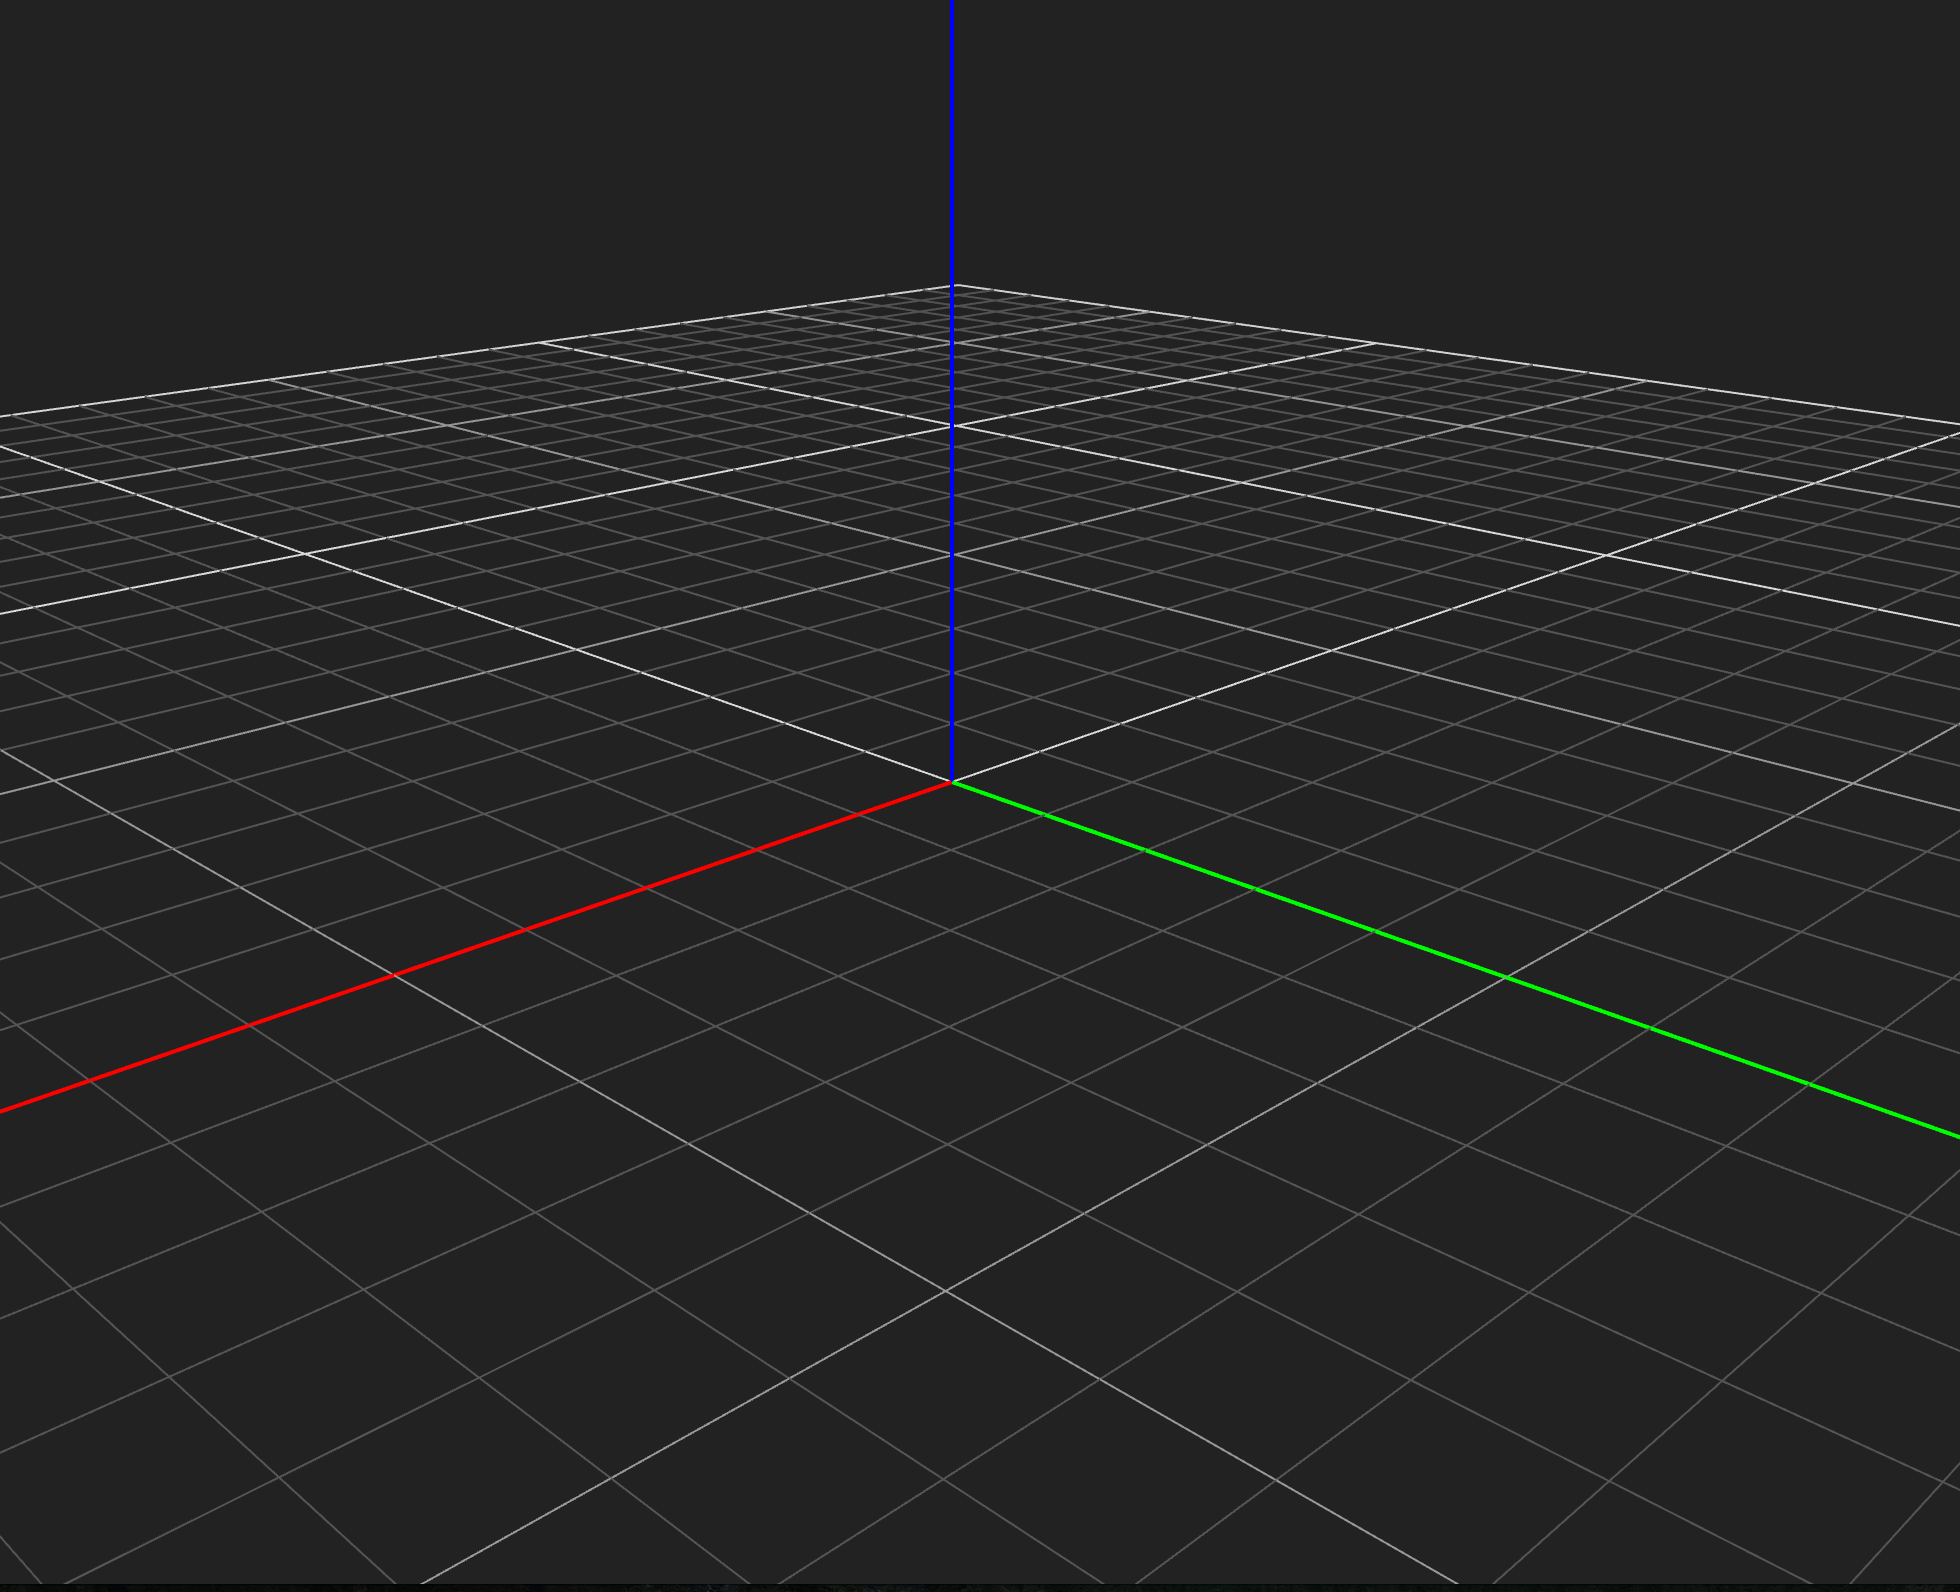
\includegraphics[width=1\columnwidth]{03-architecture_overview_coordinate_system}
  \caption{An empty scene showing the coordinate system.}
  \label{fig:architecture_overview_coordinate_system}
\end{figure}

\subsubsection{Isolated Testing Plugin}

While we developed on different stages of a sequentially
executed conversion approach in parallel, we needed a
mechanism to test each component of the conversion before
its preceeding or succeeding components were completely
implemented. The \name{IsolatedTesting} plugin provides an
isolated environment, which allows to execute a single
intermediate computation step of a conversion approach with
pre-defined input.

\subsection{The PlatenerPipeline Plugin Computes the Model
  Conversions}
\label{sec:platener-pipeline-plugin}

% - Subsection overview

The \name{PlatenerPipeline} is the main computation unit of
{\platener}. It contains algorithms and data structures to
bring the {\threedmodel} into a 2D~representation suitable
for a {\lasercutter}. Here we will outline the details about
the computation process. First we look at {\platener}'s
three conversion approaches. Then we explain the
composition of conversion approaches from computation steps
into a \class{Pipeline} data structure. Finally we present
the \class{PipelineState}, a data structure which allows to
take a snapshot of the computation state in between two
computation steps. The \class{PipelineState} is used to
render the visualizations of the \name{NodeVisualizer}
plugin.

% - needs-figure :: Pipelining Approach to subdivide the problem space
% - PipelineSteps as single computation units
% - Several Pipeline Steps make up a Fabrication Method

\subsubsection{{\platener} Presents Three Conversion
  Approaches}

The \name{PlatenerPipeline} plugin facilitates conversion
approaches. We call such a conversion approach
\class{\fabmethod}.
%A {\fabmethod} is a conversion approach of a {\threedmodel}.
It defines a linear process of analyzing a {\threedmodel}
and thereby creates a suitable equivalent of the model,
consisting of plates only. A \class{\fabmethod}
divides the conversion problem into smaller problems. Thus,
it provides a set of algorithms, which are executed
sequentially. Each algorithm solves a single subproblem. The
algorithms work on results of previously executed
algorithms. We refer to a sequence of algorithms as
\class{Pipeline}. Each algorithm in the \class{Pipeline} is
an intermediate computation step, called
\class{PipelineStep}. The first \class{PipelineStep} works
on the face-vertex mesh of the model. The last
\class{PipelineStep} returns a directly exportable data
format, in our case a {\zipfile} containing the
2D construction plans. The composition of
\class{PipelineSteps} into a \class{Pipeline} is shown in
Figure~\ref{fig:pipeline-from-steps}. \class{PipelineSteps}
are independent from the \class{\fabmethod} and thus, can be
shared between different \class{{\fabmethod}s}. {\platener}
provides three \class{{\fabmethod}s}.
% The following paragraphs present each method briefly.

\begin{figure}[h]
\centering
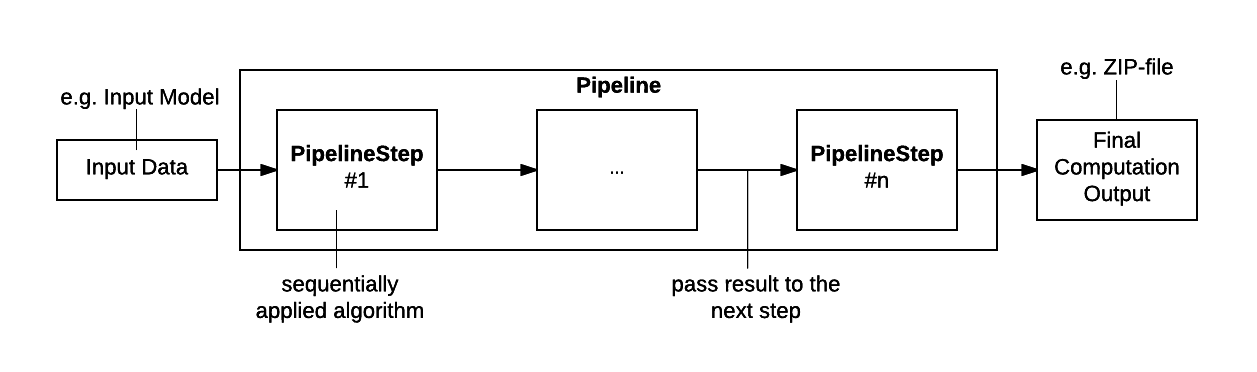
\includegraphics[width=1.1\textwidth]{03-architecture-pipeline}
\caption{A \class{Pipeline} is composed from
  \class{PipelineSteps}}
\label{fig:pipeline-from-steps}
\end{figure}

\paragraph{Plate Method}

This \class{\fabmethod} does hull and surface
reconstructions of the input model. Plates are connected via
finger joints to approximate the original {\threedmodel}.
First, the outlines of all surfaces in the model are
detected. Then, plates are formed from the outlines. For
example two parallel planar surfaces form an \name{inherent}
plate, when they are about three to five millimeters apart.
Next, plates are constructed from the remaining surfaces by
\name{extruding} the planar shapes. Then, we connect the
plates with finger joints.
Figure~\ref{fig:overview-plate-steps} depicts the important
\class{PipelineSteps} of the \name{Plate Method} and their
visualizations.

% Figure~\ref{fig:model-fingers} shows
% plates connected with finger joints.
% \begin{figure}[h]
%   \centering
%   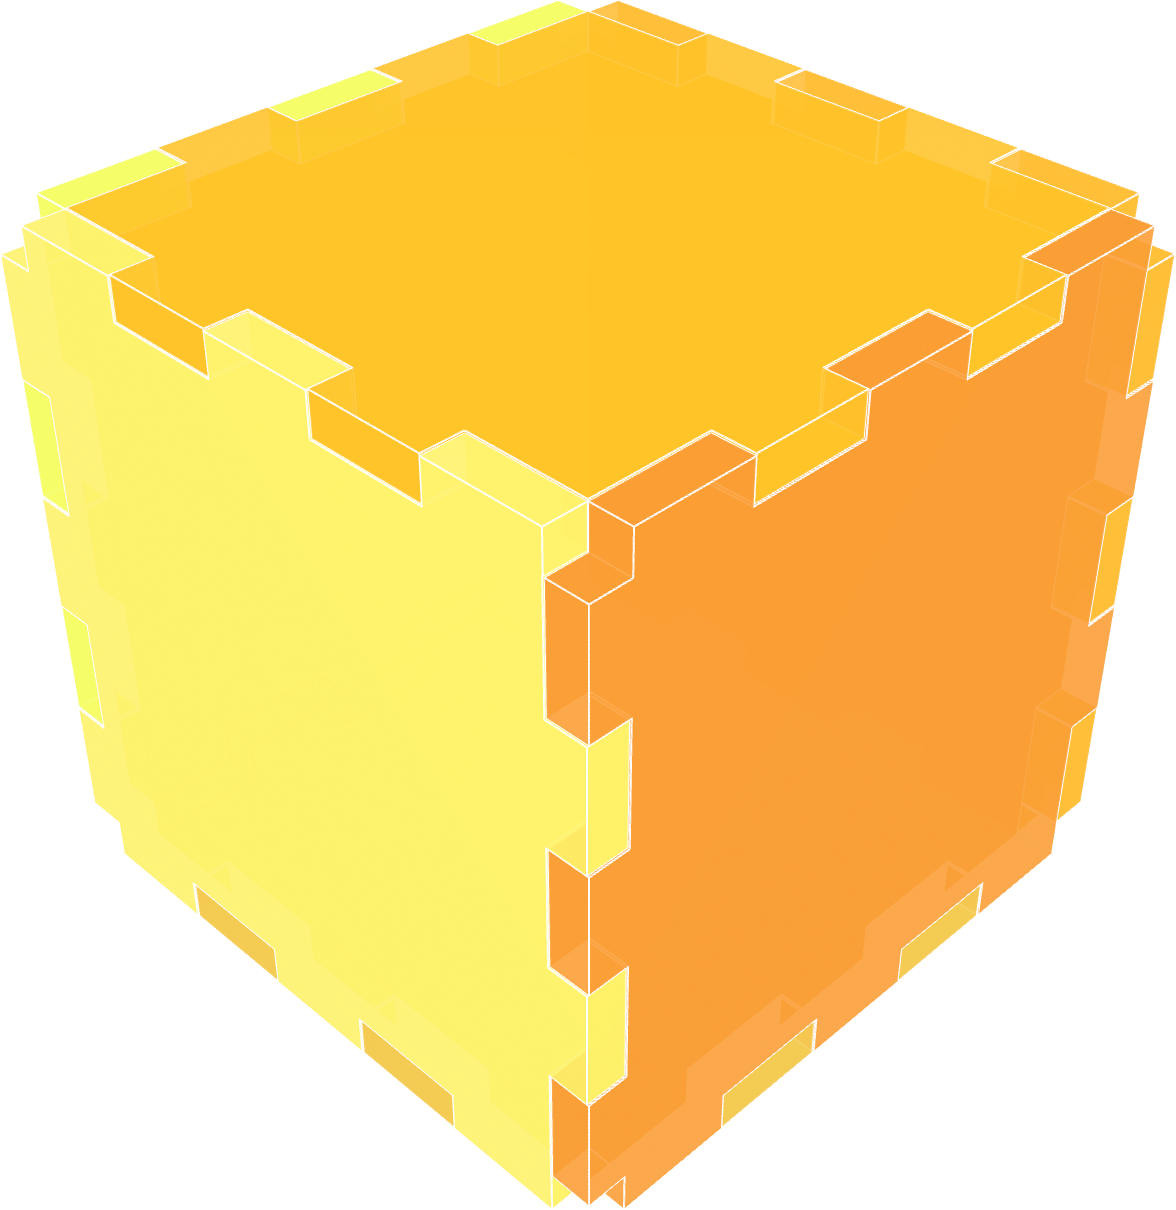
\includegraphics[width=0.6\textwidth]{03-architecture-box-fingers}
%   \caption{A model built from plates, connected with finger
%     joints.}
%   \label{fig:model-fingers}
% \end{figure}

\begin{figure}[h]
  \centering
  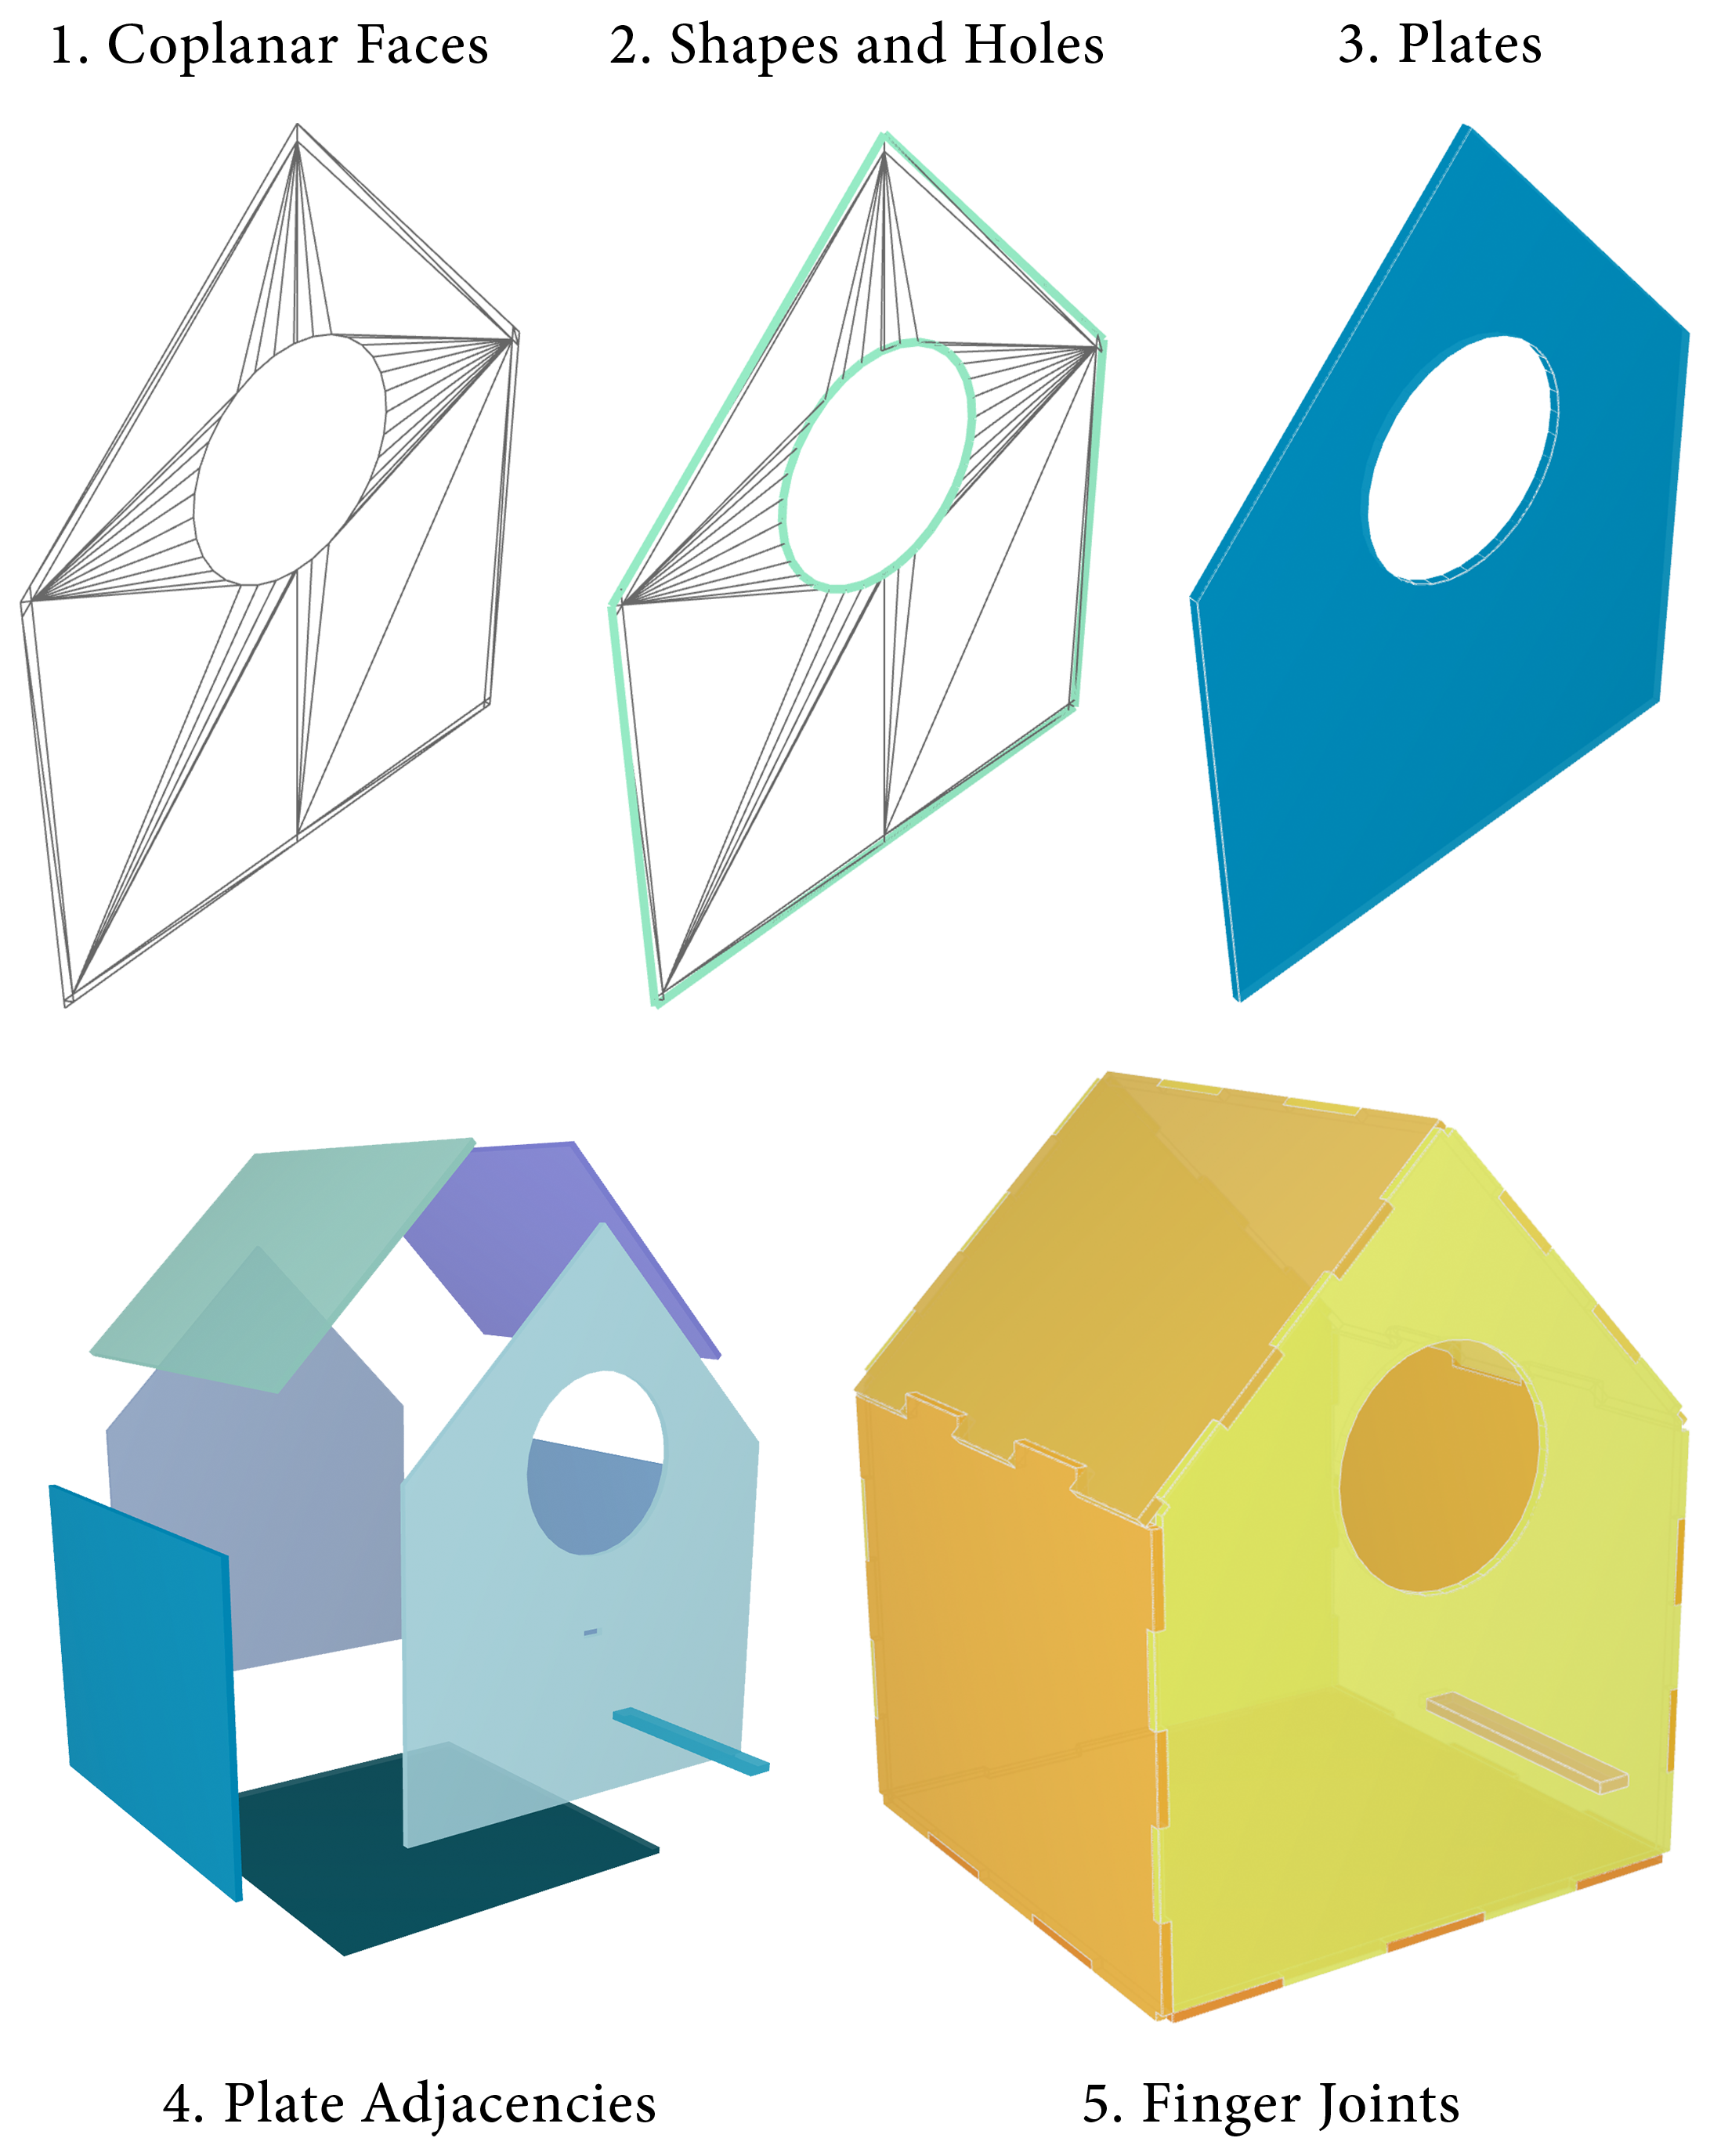
\includegraphics[width=1\textwidth]{03-architecture-pipeline-steps-overview}
  \caption{An overview of computation steps that are applied
    to the model, so that it can be built from plates.}
  \label{fig:overview-plate-steps}
\end{figure}

\paragraph{Stacked Plates Method}

This \class{\fabmethod} does volume reconstructions of the
input model. It stacks plates onto each other to approximate
the shape of the original model, see
Figure~\ref{fig:stacked-rabbit}. This preserves the look and
feel of the model. The model is sliced into equally thick
layers which form the plates. The plates are connected via
shafts to simplify the assembly process.

\begin{figure}[h]
  \centering
  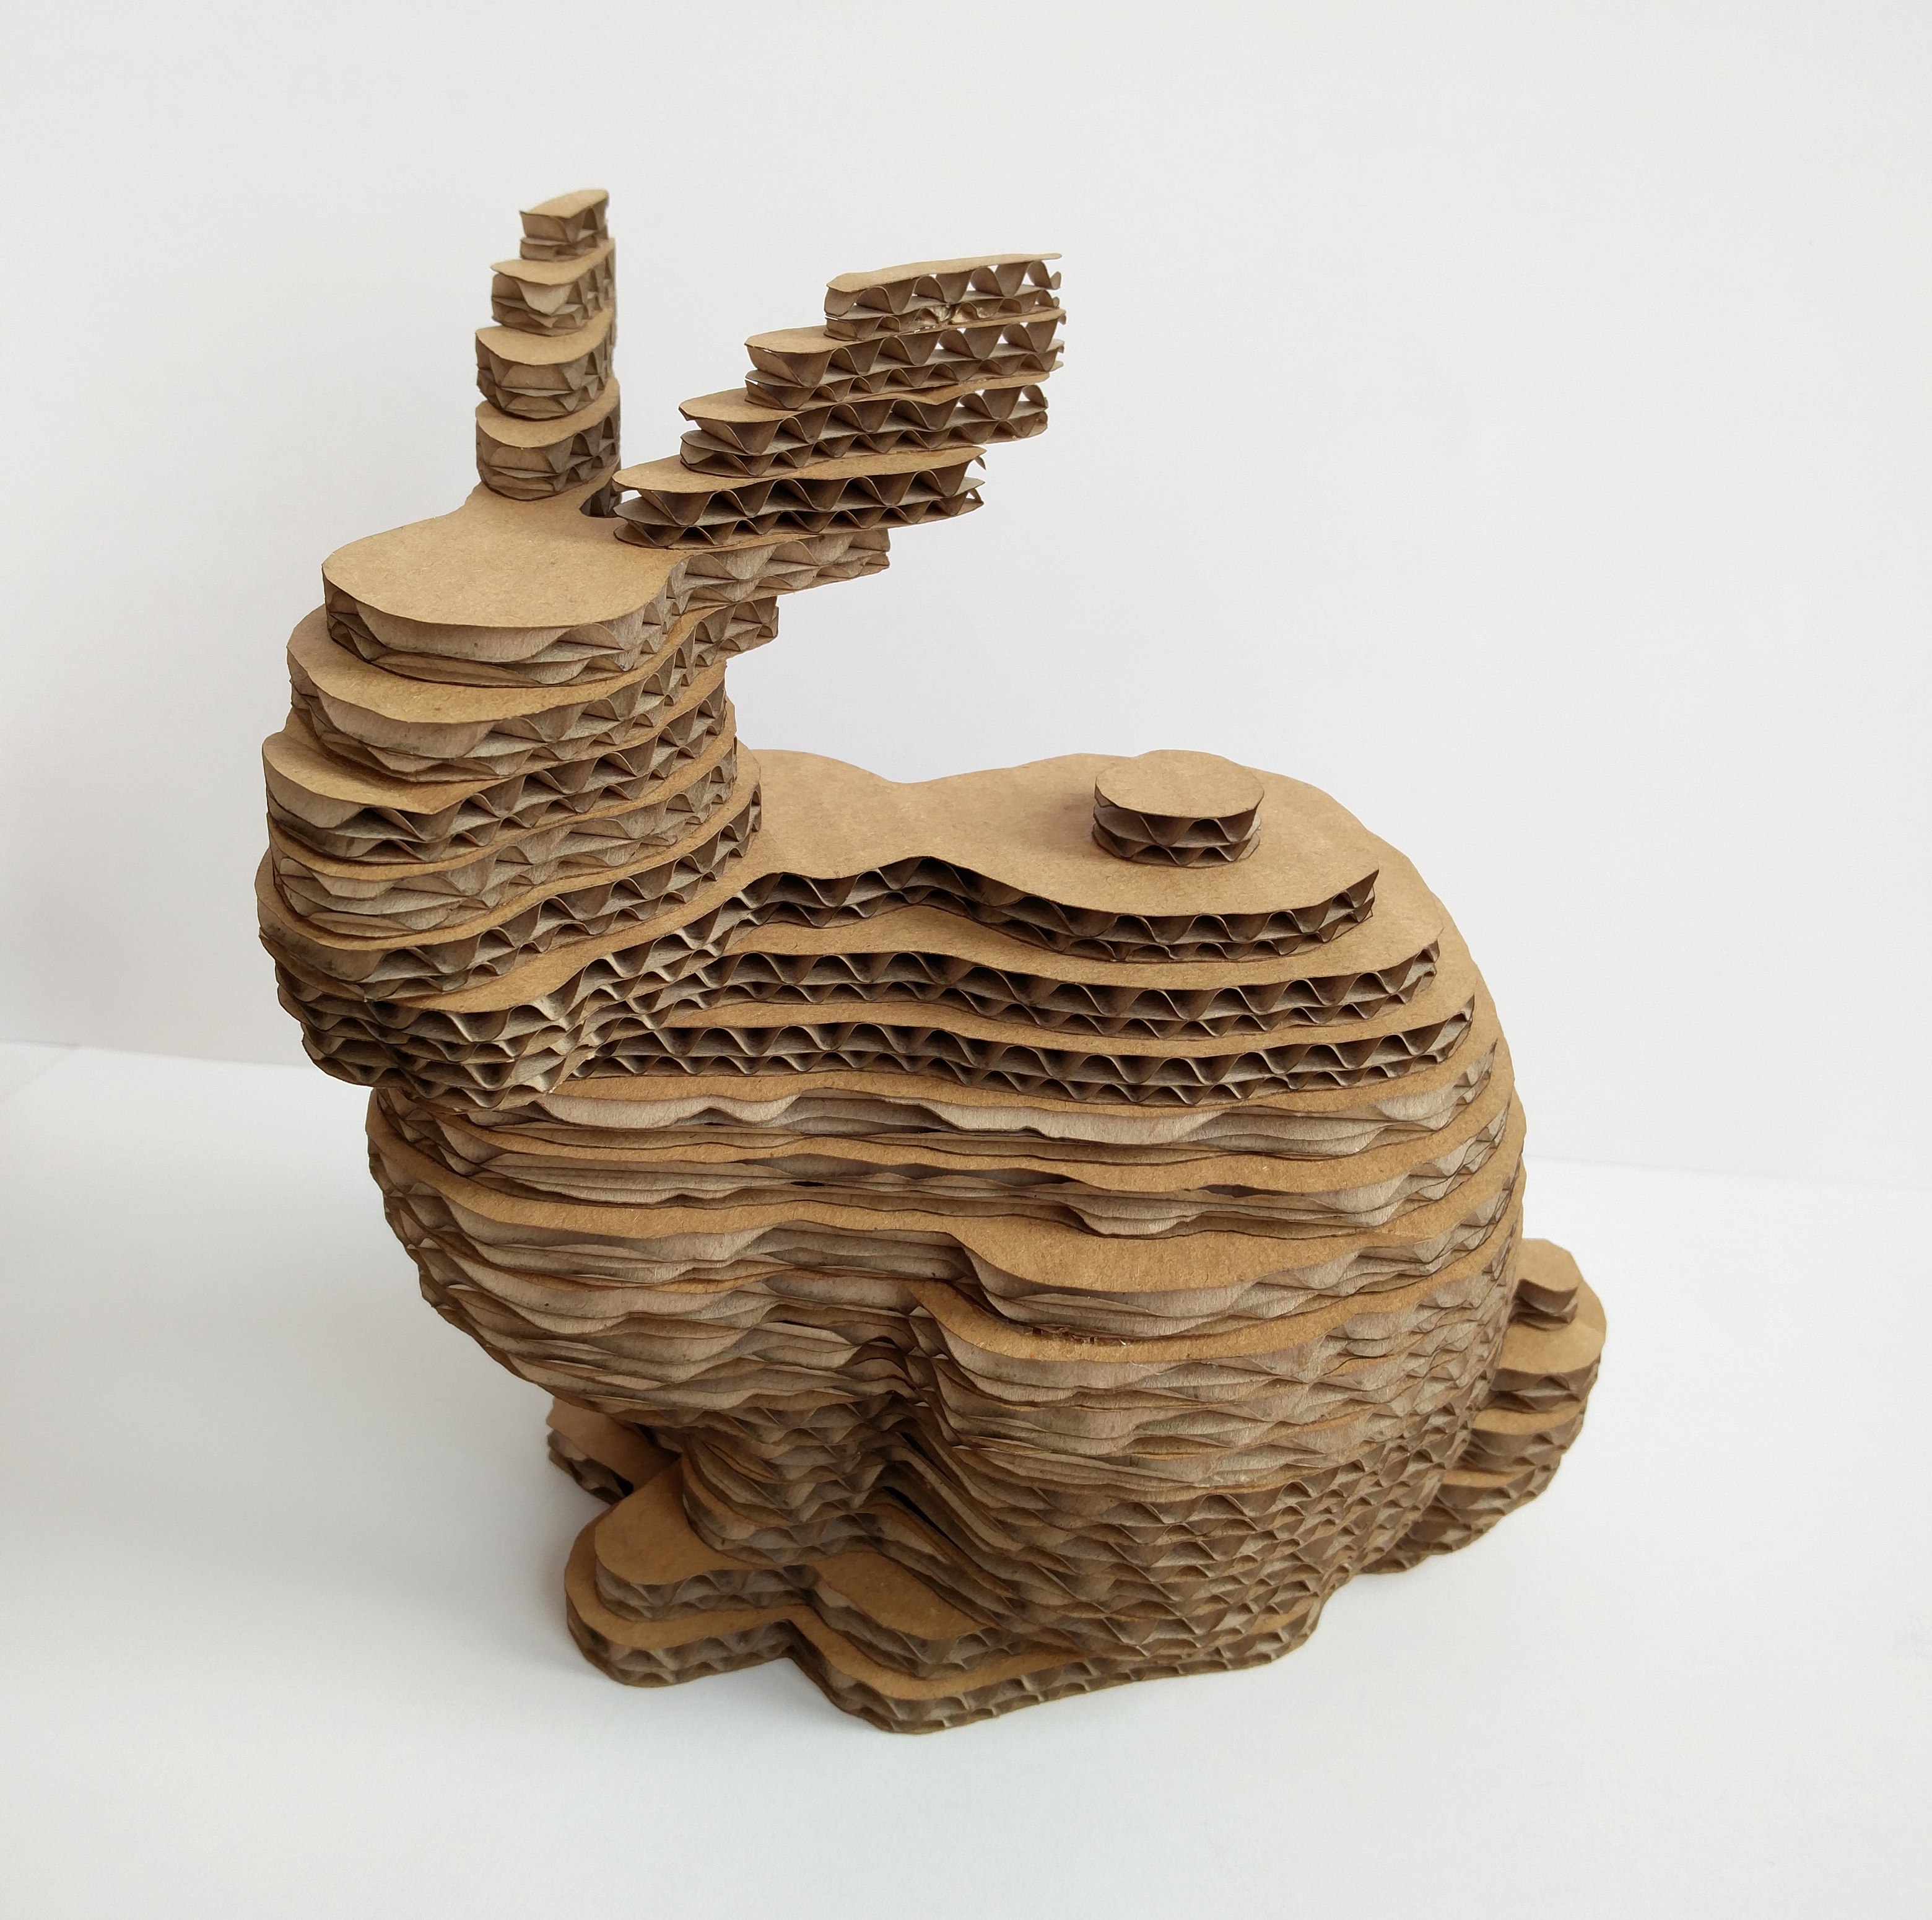
\includegraphics[width=0.6\textwidth]{03-architecture-rabbit-stacked}
  \caption{A rabbit model converted to plates with
    stacking.}
  \label{fig:stacked-rabbit}
\end{figure}

\paragraph{Classifier Method}

This is an advanced conversion approach, combining mesh
analysis and construction techniques of known geometries.
This \class{\fabmethod} will be more robust when converting
models with noisy mesh data, e.g {\threedmodel}s with lots
of texture on their surface. We analyze the model for
primitive geometries algorithms. Primitive geometries are
planes, prisms, boxes, cylinders or spheres.
Figure~\ref{fig:tiki-cylinder} shows the classification of a
cylinder in a model using a non-deterministic algorithm.
These geometries can be combined to high-level
representations of the input model, giving more information
than a mesh of triangles. The model is structured into an
hierarchical graph consisting of these primitive geometries
only. It is similar to a scene graph. For each of these
primitives we know a conversion approach to plates which
will give better results than approximating a set of faces.
The \name{Classifier Method} is a proposal and part of
future work. We can currently classify a subset of the
primitive geometries.

\begin{figure}[h]
  \centering
  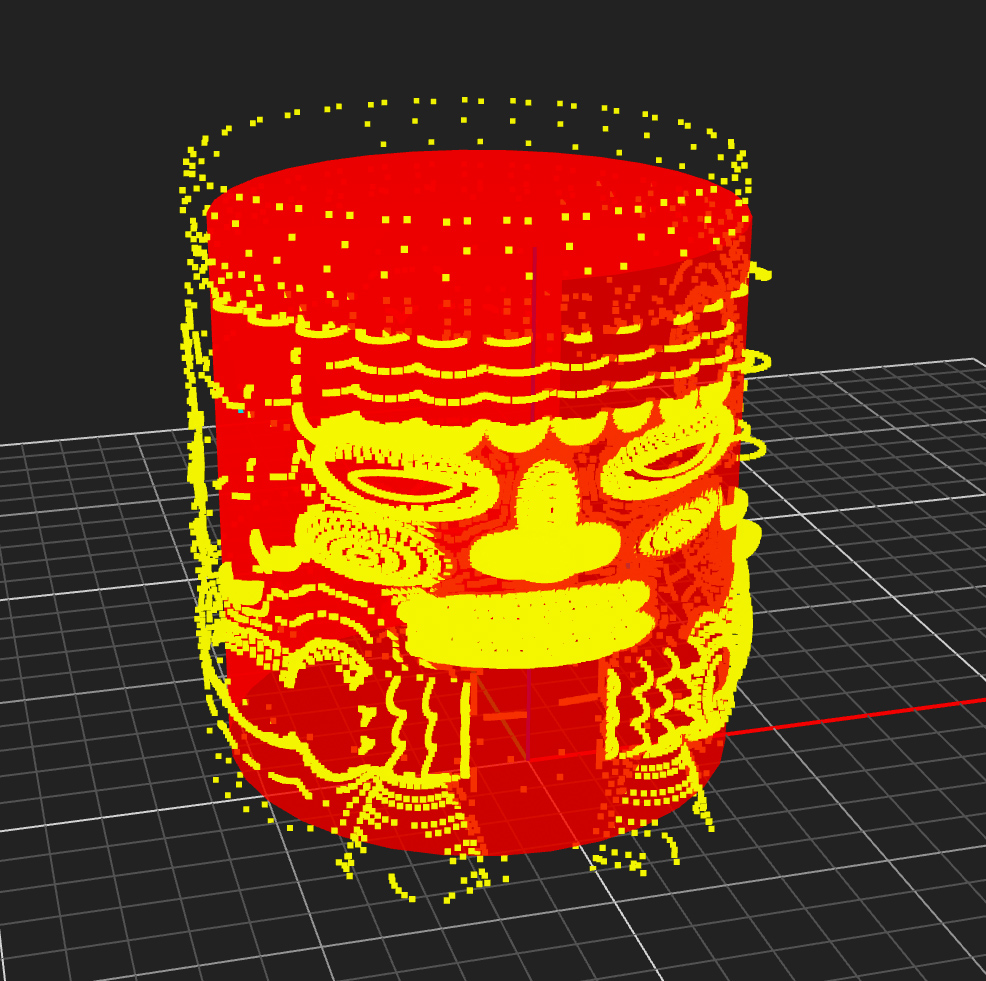
\includegraphics[width=0.6\textwidth]{03-architecture-tiki-cylinder}
  \caption{A classified cylinder in a model with textures.
    The yellow points, show the outline of the actual model.}
  \label{fig:tiki-cylinder}
\end{figure}

\subsubsection{Pipeline Steps Compute Cloneable States}

Each \class{\fabmethod} assembles a \class{Pipeline} from
\class{PipelineSteps}. \class{PipelineSteps} work on the
data of previous computation steps and pass the data to the
next compution steps. To improve the development and
debugging experience we preserve a snapshot of the data. We
call the state of a given data structure at a given point in
time a snapshot. A snapshot of the computed data is used to
render a visual representation of the data. The visual
representation gives a clear understanding of the data and
thus, enhances the development and debugging experience.
Note, that the \class{PipelineSteps} are merely computation
units. All visual output is done in the
\name{NodeVisualizer} plugin.

The data that is passed between the \class{PipelineSteps} is
encapsulated in a \class{PipelineState}. The
\class{PipelineState} contains all data structures that are
ever to be computed by all \class{PipelineSteps}. It is
essentially a container for every computation result.

The \class{PipelineState} is a cloneable data structure. A cloneable
data structure can be copied. When the algorithm of a
\class{PipelineStep} finishes, the \class{Pipeline} writes the results
into the \class{PipelineState}. A snapshot is obtained by cloning the
\class{PipelineState} after the execution of a \class{PipelineStep}.
Figure~\ref{fig:pipeline-with-snapshots} illustrates how snapshots are
obtained between the \class{PipelineSteps}.

\begin{figure}[h]
  \centering
  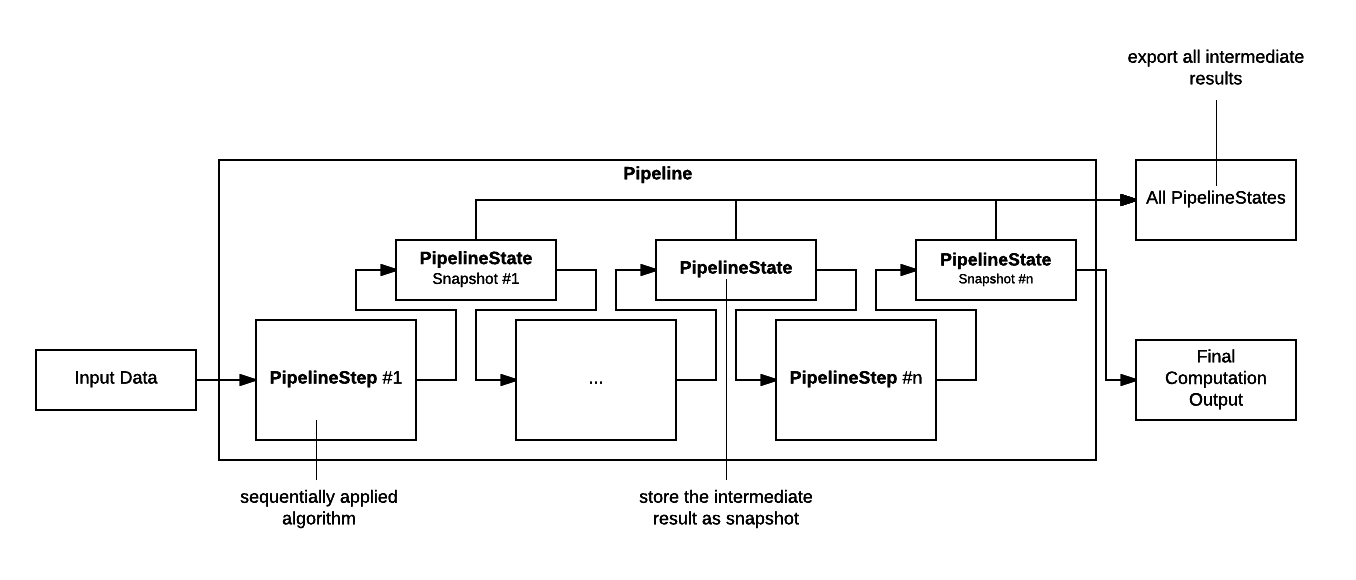
\includegraphics[width=1.1\textwidth]{03-architecture-pipeline-with-snapshots}
  \caption{The pipeline preserves deep copies of intermediate computation results.}
  \label{fig:pipeline-with-snapshots}
\end{figure}


The encapsulated data in the state can contain multiple
fields and can be hierarchical. We provide a fully cloneable
data structure. That means, any nested data structure in the
\class{PipelineState} implements a cloneable interface
%and supports copying as well.
The clone of an instance of \class{PipelineState} is a
deep copy.

A deep copy of a data structure is a clone of all fields and
recursively the nested fields of all fields of that data
structure. That means if a data structure references
dynamically allocated memory, we do not clone the reference
of the allocated memory to the copy of the data structure.
Instead, we allocate new memory and duplicate the data to
the newly allocated memory. Thus, we make sure modifications
on the copy do not alter the original.

When we take a snapshot of the results of a
\class{PipelineStep} we ensure that modifications of a
subsequent \class{PipelineStep} will not alter the data in
the snapshot of a previous \class{PipelineStep}. Otherwise,
the \name{NodeVisualizer} plugin would render corrupted
visuals for the previous step. Figure~\ref{fig:corrupt}
shows how the surface reconstruction step would be effected
by the creation of finger joints, when \class{PipelineSteps}
are not deep clones. Figure~\ref{fig:corrupt:shapes} shows
the edges of the cube. These edges are mutated in order to
attach new finger joint geometry. The final finger joints
are depicted in Figure~\ref{fig:corrupt:fingers}. When the
edges data structure is not copied before adding the finger
joints, the edge visualization will also show the finger joints
(Figure~\ref{fig:corrupt:shapes-fingers}).

\begin{figure}[h]
  \centering
  \begin{subfigure}[b]{0.3222\textwidth}
    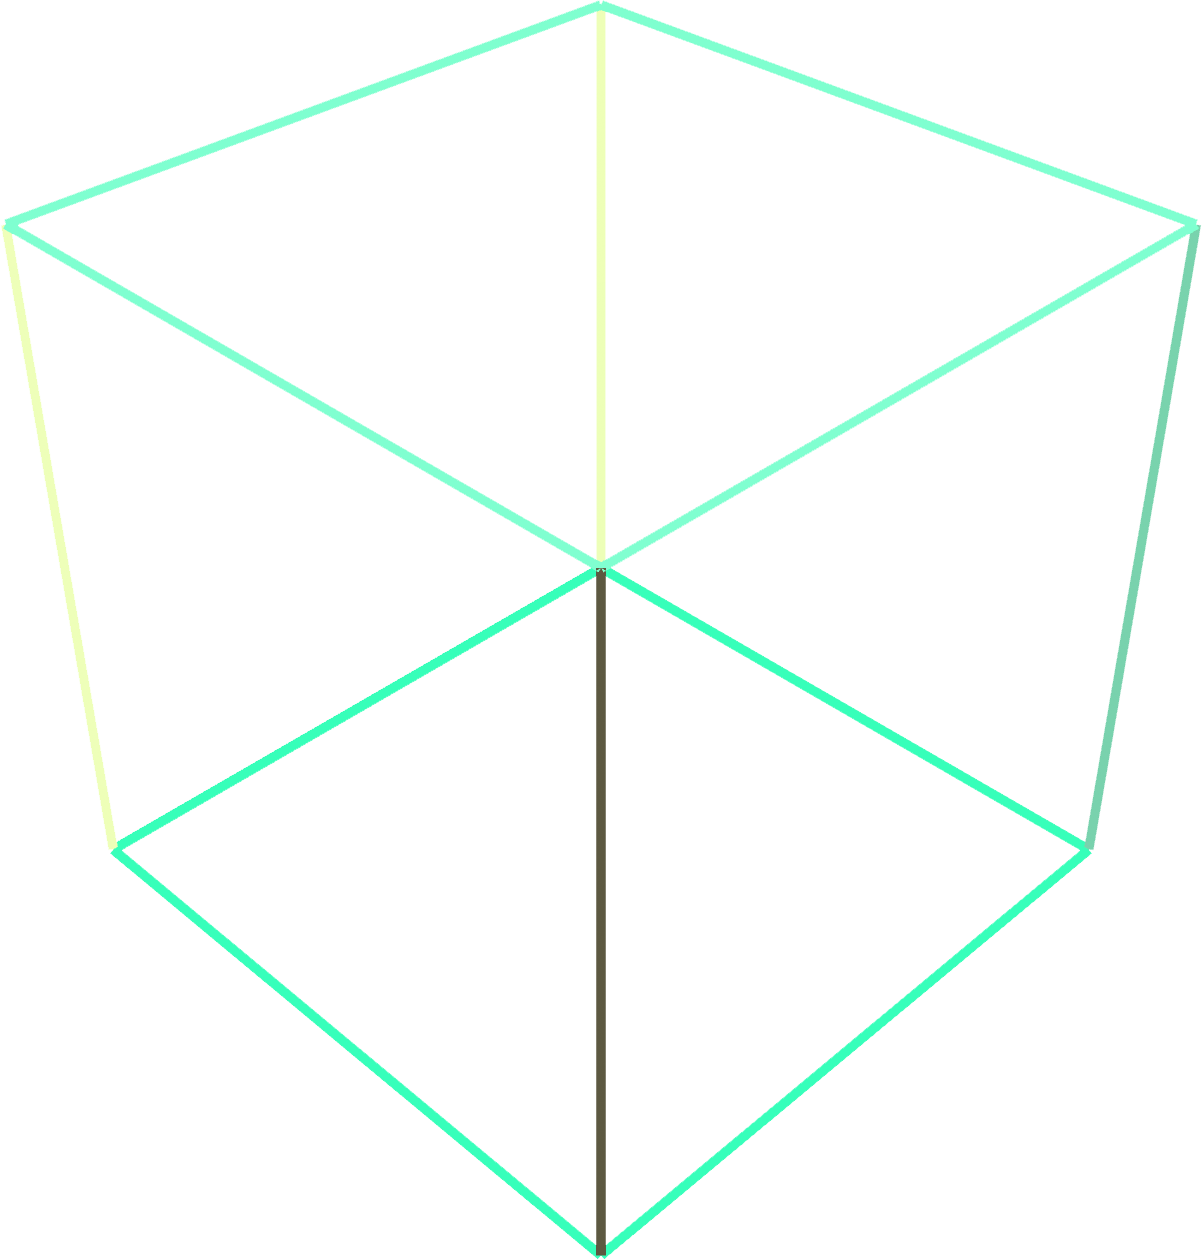
\includegraphics[width=\textwidth]{03-architecture-box-shapes}
    \caption{The shapes of a box.}
    \label{fig:corrupt:shapes}
  \end{subfigure}
  \begin{subfigure}[b]{0.3222\textwidth}
    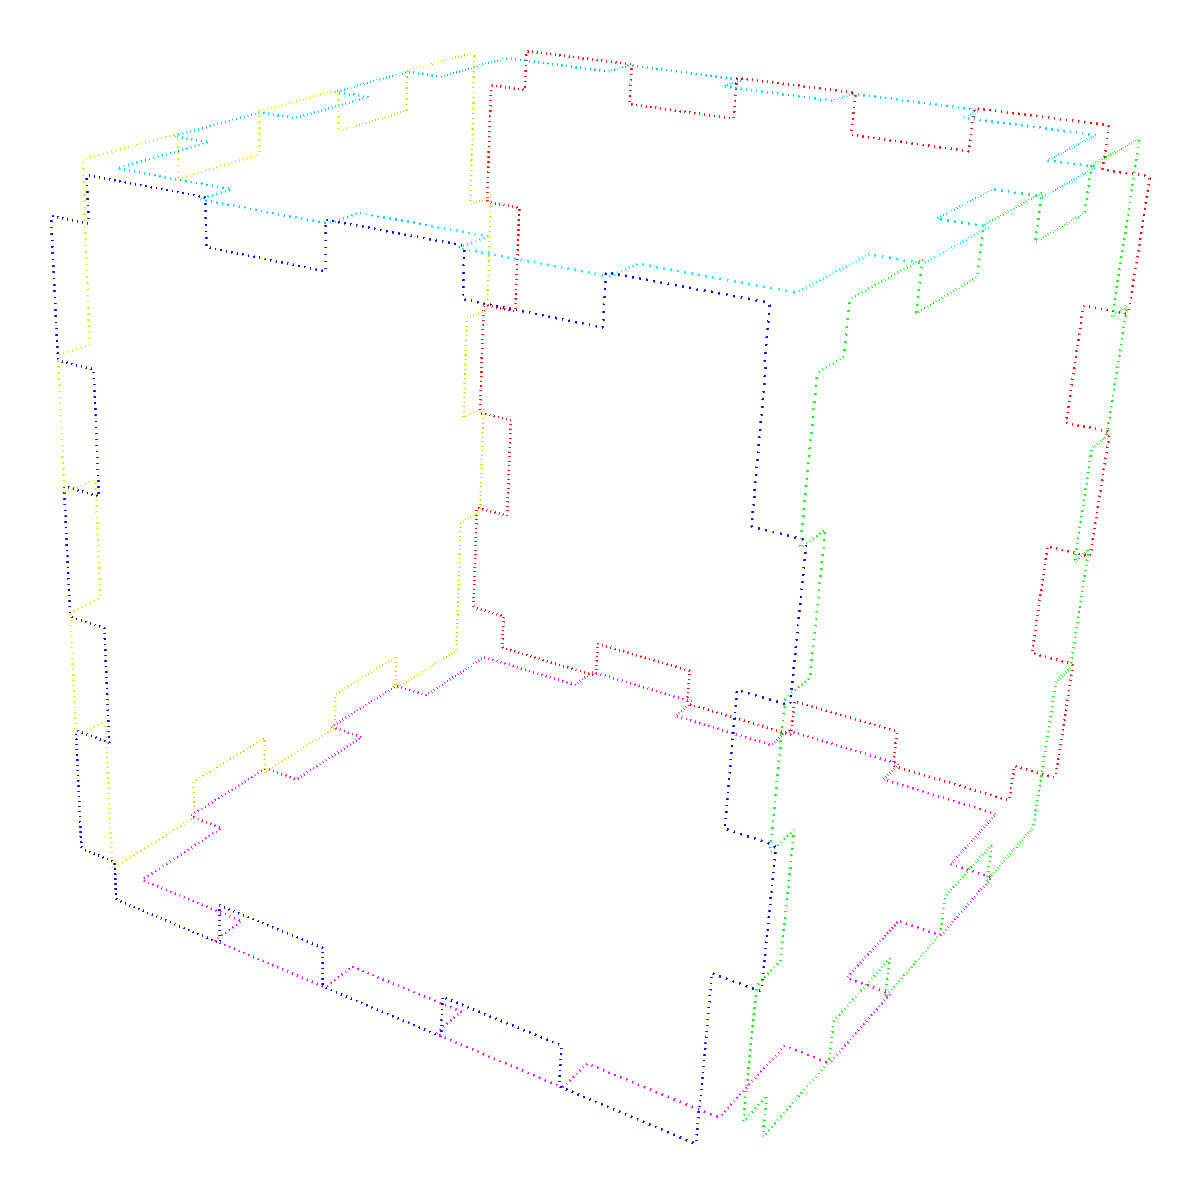
\includegraphics[width=\textwidth]{03-architecture-box-shapes-with-fingers}
    \caption{Corrupted shapes of a box, showing the finger joints.}
    \label{fig:corrupt:shapes-fingers}
  \end{subfigure}
  \begin{subfigure}[b]{0.3222\textwidth}
    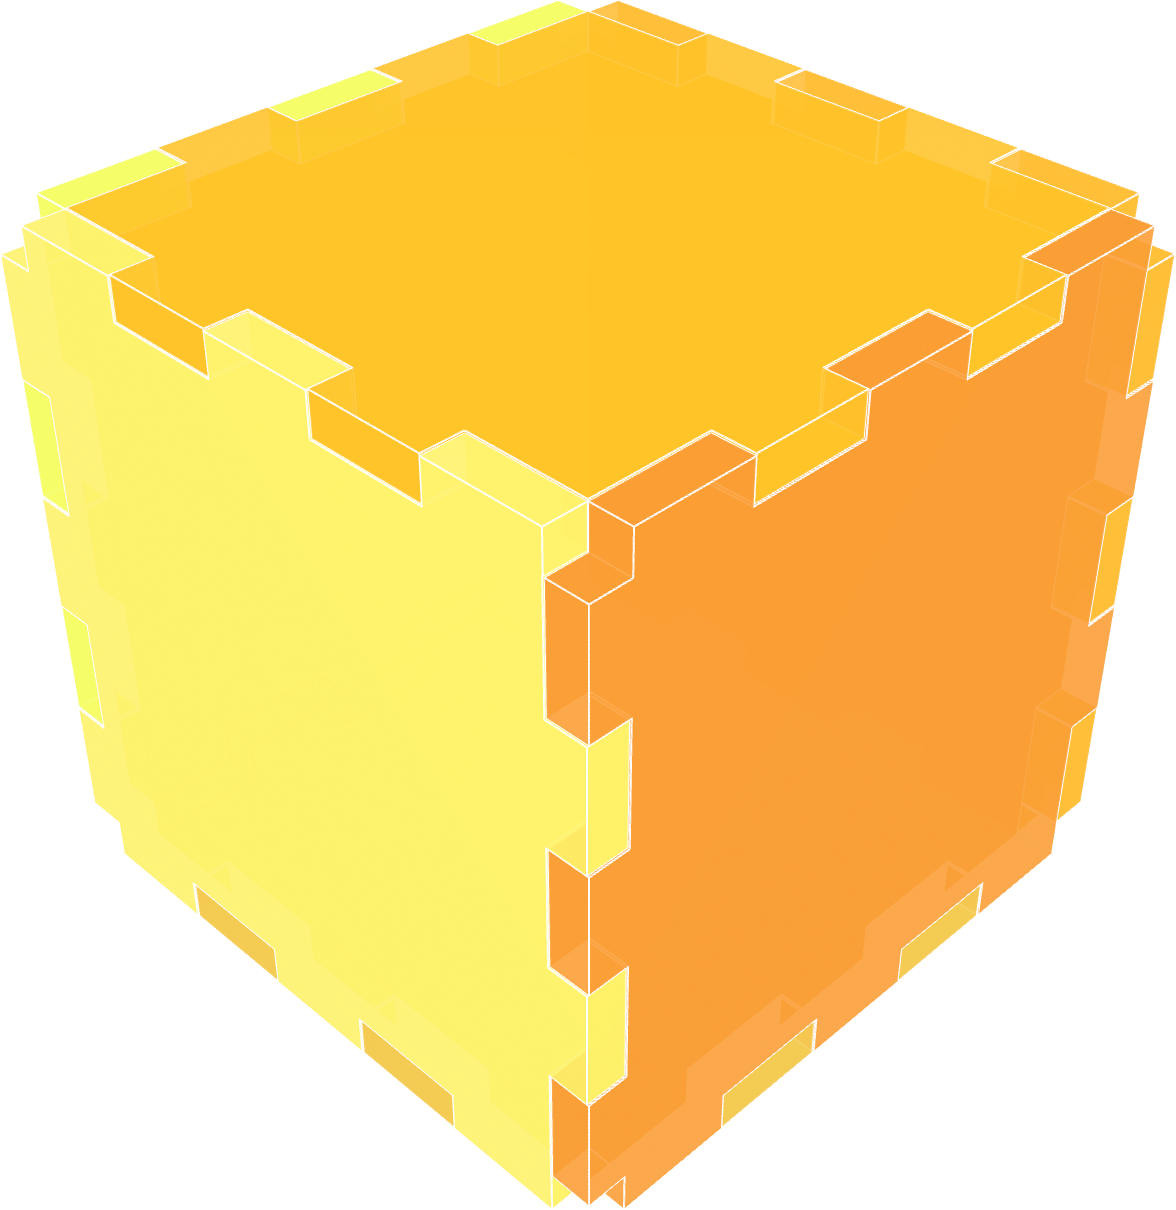
\includegraphics[width=\textwidth]{03-architecture-box-fingers}
    \caption{A box with finger joints.}
    \label{fig:corrupt:fingers}
  \end{subfigure}
  \caption{Modifications to shallow copies of the data
    corrupt the visualizations.}
  \label{fig:corrupt}
\end{figure}


% \item Pipeline Implementation

%   \begin{enumerate}
%   \item the pipeline works as follows...
%     \begin{itemize}
%     \item Pipeline class
%     \item pipe interface for Step factories (compare listing above, stacked method)
%     \item create state factory -> use composition to persist intermediate results
%       (state is later accessed by node visualizer)
%     \item reduce approach -> pipe last state into next step to produce new state
%     \item show a listing of pseudo code, explaining how the pipeline works
%     \item benchmarking (measure time for intermediate steps vs whole processing)
%     \end{itemize}

%   \item it can be reused (because pipelining is a generic concept)
%     \begin{itemize}
%     \item classifier graph (classification method)
%     \item isolated testing (injectable pipeline)
%     \end{itemize}
%   \end{enumerate}

% \end{enumerate}


\subsection{Code Packages of {\platener}}
\label{sec:code-packages-platener}

% - Subsection overview

% This section describes the code packages of {\platener}.
% Furthermore, we explain how {\convertify} is used by
% {\platener} and how the user interface is connected to the
% plugins.

%     - needs-figure :: Application is separated into
%     Packages


\begin{figure}
  \centering
  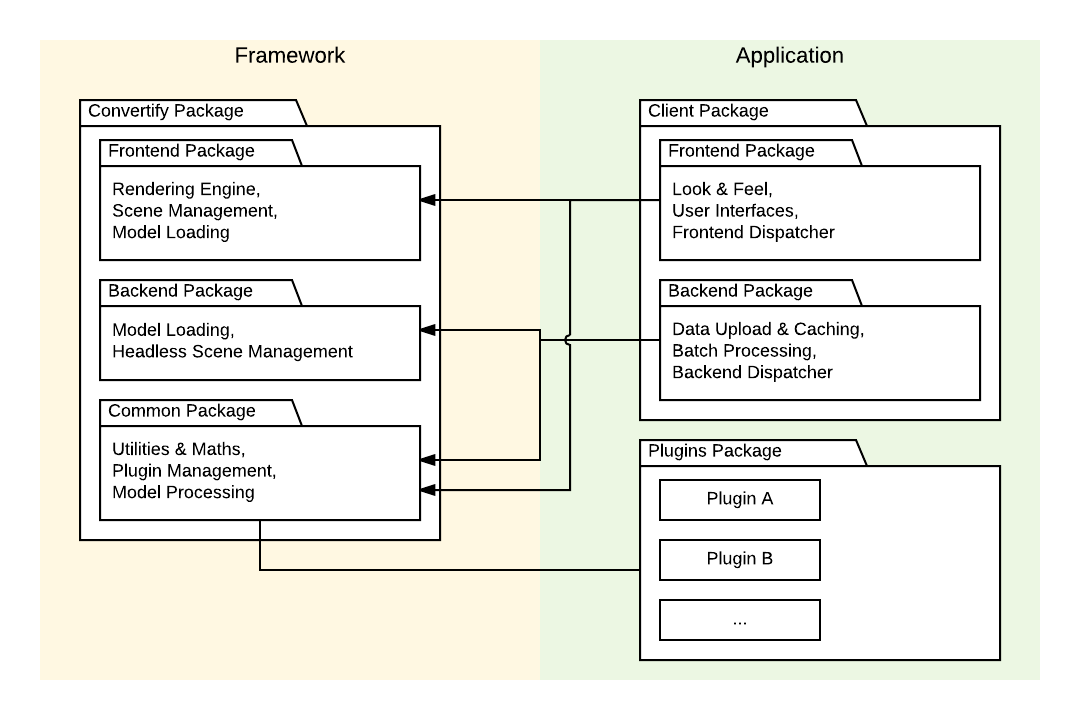
\includegraphics[width=1.1\columnwidth]{03-architecture-package-diagram}
  \caption{Main Packages of the Platener Architecture}
  \label{fig:package-diagram}
\end{figure}

{\platener} is divided into the code packages {\convertify},
plugins and client. Figure~\ref{fig:package-diagram}
shows the detailed package diagram. Each package takes over a set of distinct
responsibilities. The {\convertify} package is the framework,
described above. The plugins package provides an exchangeable
set of features for the WebGL scene. The client package gives
the look and feel of {\platener}. It provides user interfaces for the
web application in the frontend package and a command line interface
in the backend package.

The {\convertify} code package was described in detail in
Section~\ref{sec:framework-convertify}.

The plugins package contains seven plugins, where each plugin is a
separate subpackage. The plugins implement the computational and
render logic of {\platener}. We introduced these plugins in
Section~\ref{sec:platener-uses-plugins}.

%     - We have a WebApp and a Server package, which are both Client
%       code, because we have two types of applications
%     - the WebApp is an online service deployed for use by Makers

The client package of {\platener} is twofold. It contains a
subpackage for the frontend and backend application. The
frontend application enables users to convert
{\threedmodel}s to laser cuttable files in their web
browser. The web application is build with React components.
React is a {\javascript} library for building user
interfaces. We will introduce React and our React setup in
Section~\ref{sec:ui-with-react}. The backend application is
a command line interface running on {\nodejs}. With the
backend application users can batch-process a set of models
without using a browser. We give details about the CLI-tool
in Section~\ref{sec:cli-tool}. Also, we provide a server
which manages a repository of {\threedmodel}s and their
conversions.

\subsection{The Frontend Package Connects Plugins and User Interfaces
  Into a Web Application}
\label{sec:client-to-application}


% **** The WebApp Package Builds a Cross-platform Web Page

%      - Subsubsection overview
%      - needs-ref :: Web Interfaces are built with HTML and CSS
%      - needs-ref :: The React library | copy from AOP paper
%      - needs-ref, needs-figure :: The Redux library (Dumb Components and Smart Containers)
%      - needs-figure :: Using Redux dispatch in the Dispatcher
%      - Subsubsection summary


The frontend package bundles React components, building the web
application's user interface. It accesses {\convertify}'s
\class{Bundle} to control the rendering engine and scene
management as well as loading the plugins. We implement a
\class{Dispatcher} in the frontend package which connects the plugins
with the {\userinterface}.

\subsubsection{Building User Interfaces With the React Library}
\label{sec:ui-with-react}

React provides a powerful tool to build user interfaces for web and
mobile applications \cite{React13}. As React is currently under active
development the growing user base emphasizes its practical
relevance\footnote{\url{http://facebook.github.io/react/blog/2015/03/30/community-roundup-26.html}}.

React provides a virtual DOM consisting of lightweight representations
of DOM nodes, called \name{Components} \cite{React13}. A Component is
stateful and provides behavior, e.g. manages click interaction by a
user. With focus on flexibility React allows composition of
Components. Multiple Components may be nested into a parent Component.
The parent Component passes state onto its children. Children can
notify their parents by emitting events or executing callbacks. In
short, in React data is passed from parent to children, while the
event flow is directed from children to parent
\cite{ReactDocComponents}. To enhance code readibility, React
introduces the {\javascript} Syntax Extensions
(JSX)\footnote{\url{https://facebook.github.io/jsx/}}. This code
transpilation allows the usage of HTML-tag syntax to instantiate
compositions of Components. As our setup is based on {\coffeescript},
we use a {\coffeescript} variant of JSX, called
CJSX\footnote{\url{https://github.com/jsdf/coffee-react-transform}}.
Listing~\ref{lst:react-snippet} shows a React Component containing a CJSX
snippet.

\begin{listing}[h]
\begin{minted}[
linenos
]{coffeescript}
# instantiate a React Component
RootComponent = React.createClass
  # put this HTML-snippet into the DOM,
  # when displaying this component
  render: ->
    return (
      <section className="root">
        {@props.children}
      </section>
    )
\end{minted}
\caption{A {\coffeescript} example showing a root component, wrapping
  its children into an HTML-tag with a class name.}
\label{lst:react-snippet}
\end{listing}

The real DOM is re-rendered as soon as React detects changes in the
virtual representation of the DOM. This is done with reactive updates.
This means the \textit{render} method of a Component is invoked again,
when the Component's data changes. This causes React to \enquote{throw
  away the entire UI and re-render it from
  scratch}\footnote{\url{http://www.quora.com/How-is-Facebooks-React-JavaScript-library/answer/Lee-Byron?srid=3DcX}}
\cite{React13}.


\subsubsection{Managing Data Flow of React Components with the Redux
  State Container}
\label{sec:flow-with-redux}

Redux\footnote{\url{http://redux.js.org/}} is a {\javascript} library
which aims to reduce complexity when managing state of frontend
components with React. As each React Component is stateful, keeping
track of state and updating state in the asynchronous browser
environment is cumbersome. With Redux we manage all state of our
frontend application in one place, resulting in \enquote{a single
  source of truth} \cite{redux}. This state is a read-only object
tree called \name{store}. All mutations to the store have to be applied by
actions. An action is a plain object comprising the intent of
mutating the state \cite{redux}. Listing~\ref{lst:action-dispatch}
shows such an action.

\begin{listing}[h]
\begin{minted}[
linenos
]{coffeescript}
store.dispatch({
  type: 'CHANGE_PLATEFINDING_ALGORITHM'
  algorithm: 'INHERENT_AND_EXTRUSION'
})
\end{minted}
\caption{A state change to the store, indicating which plate finding
  algorithm is selected in the user interface.}
\label{lst:action-dispatch}
\end{listing}

The intended state change of an action is propagated by a
reducer. Every reducer is a pure function. A pure function
has no side effects. A reducer applies a data transformation
on the state tree. Listing~\ref{lst:action-reducer} shows a
sample reducer which changes the state according to the
selected algorithm. The pipeline reducer checks for
the dispatched action and creates a new state object with the
selected algorithm.

\begin{listing}[h]
\begin{minted}[
linenos
]{coffeescript}
initialState =
  platefindingAlgorithm: DEFAULT_PLATEFINDING_ALGORITHM

pipeline = (state = initialState, action) ->
  switch action.type
    when CHANGE_PLATEFINDING_ALGORITHM
      return Object.assign(
        {}
        state
        { platefindingAlgorithm: action.algorithm }
      )
    else return state
\end{minted}
\caption{A reducer applies state transformation of actions.}
\label{lst:action-reducer}
\end{listing}

When the state is changed by a reducer each React Component
that uses data from the changed portion of the state is
updated. A re-render is triggered. Thus, we emphasize a
purely data-driven update flow in our frontend application.
This brings explicit dependencies and avoids race conditions
\cite{redux}.

\subsubsection{A Dispatcher Connects {\convertify} With the User
  Interface}
\label{dispatch-and-dispatcher}

%     - needs-figure :: Client code connects all plugin
%     features with a user interface

%     - Use Framework to wire up everything, but not part of the
%       framework (Bundle and Protocols come in handy, Client code
%       implements a Dispatcher instance = the mediator)

{\convertify} decouples any user interface specific code
from the actual logic and rendering. We can observe the
state of {\convertify} by listening to events. In this
section we describe how the events of {\convertify} are
propagated into our web interface. As all {\userinterface}
is setup in a Redux store we have a purely data-driven
approach to update the user interface. That means, changes
from within {\convertify} have to be propagated to the Redux
store. Changes to the store are applied through actions.
Each state change of {\convertify} is mapped to a Redux
action. This mirrors the change of state from {\convertify}
to the frontend. For example, when the
\name{PlatenerPipeline} plugin finishes the computation of
laser cutter conversions, the \class{Dispatcher}'s
\name{evaluationDidFinish} callback is invoked.
Figure~\ref{fig:dispatcher-dispatch} shows how the
\class{Dispatcher} and Redux are connected. The
\class{Dispatcher} has access to the Redux store. This is
possible because the \class{Dispatcher} is implemented in
the frontend package. It uses the store's
\name{dispatch} method and an action to propagate the
solutions to Redux. Now, we still have a fully data-driven
approach connecting our framework with {\platener}.

\begin{figure}
  \centering
  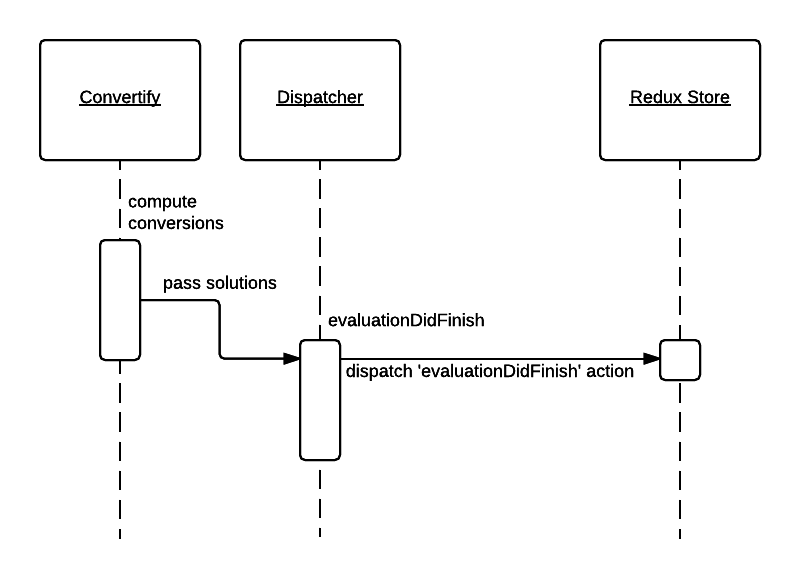
\includegraphics[width=1.1\columnwidth]{03-architecture-dispatcher-dispatch}
  \caption{The \class{Dispatcher} connects {\convertify} and the Redux store.}
  \label{fig:dispatcher-dispatch}
\end{figure}

\subsection{The Backend Package Provides a Command Line Interface for
  Batch Processing}
\label{sec:cli-tool}

%     - the CLI tool is a service for batch processing or integration
%       with other applications

% **** The Server Package Allows Headless Batch Processing of Models

%      - Subsubsection overview
%      - A CLI tool runs in nodejs
%      - needs-ref :: Processing objects without opening a browser (isomorphic code)
%      - Processing multiple objects in sequence
%      - Integration with tools to be built in future
%      - Subsubsection summary


The backend package of {\platener} provides a command line interface
(CLI). With the CLI of {\platener} we can process multiple
{\threedmodel}s in a queue. Results are read from and stored in
a directory. We receive detailed summaries and logs for each
conversion. A walkthrough of our CLI is given in
Section~\ref{sec:walkthrough-cli}.

A command line interface is an application solely consisting of
textual input and output. A CLI is typically more flexible and
powerful than a graphical user interface. Because a CLI has to be used
in a terminal window, it targets mostly advanced users. Another upside
of CLIs is that they can be integrated within other applications,
e.g. when executing shell commands \cite{cli}.

Performing a single conversion at a time is sufficient for most
users. Using a web interface for that task makes it as easy as it can
get. Though when dealing with a collection of objects the manual
conversion of each model is cumbersome. Our CLI provides a batch
processing method by reading data from the local file system. For each
{\stlfile} the CLI starts the \name{PlatenerPipeline} and writes the
output to a {\zipfile} into a target directory. Similar to the
frontend package we implement a \class{Dispatcher} instance which
connects the CLI commands and actions to {\convertify}.

When a conversion finishes we log details of the progress.
Figure~\ref{fig:reports} shows the variety of available
reports. We only store the conversion's meta data into a
\class{Report} instance. The garbage collector of the
{\javascript} engine frees the occupied memory of the
{\threedmodel}. The \class{Reports} are printed to the
console after all conversions finish. On top of the
individual report per object we summarize all data and give
a brief statistical overview.

\begin{figure}
  \centering
  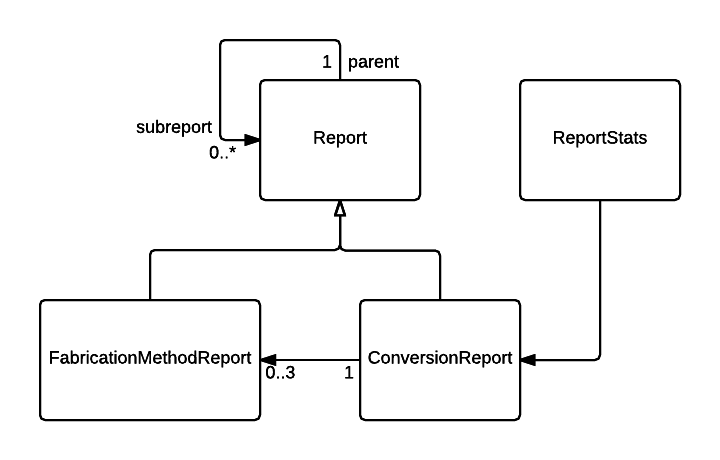
\includegraphics[width=1.1\columnwidth]{03-architecture-reports}
  \caption{The CLI logs reports for each conversion.}
  \label{fig:reports}
\end{figure}

% A CLI can be controlled via a shell. This makes it easy, to integrate a
% CLI into another application. Thus, {\platener} could be used by other
% 3D-editors to generate laser cutter conversions in an interactive
% environment.









% \subsection{Package Responsibilities}

%  ensuring decoupled
% components. Thus a flexible, maintainable system is created.

% \emph{Convertify} provides generic tools which support plugins in manipulating
% {\threedmodel}s. This includes utilities for vector analysis as well as
% rendering routines and scene management. The application lifecycle can be
% initiated and observed via a \emph{Bundle}. A Bundle represents an instance of
% the application's computation unit. The Client and Server packages run a Bundle.

% \emph{Plugins} provide an exchangeable set of features which are used by the
% Client and Server package. A Plugin interacts with the Scene and its
% {\threedmodel}s via lifecycle events. E.g. a concrete conversion strategy
% provided by Platener is implemented by a single Plugin. Plugin features can be
% enabled for Client, Server or both.

% The \emph{Client} package gives the look and feel of the application. This
% package contains frontend components. The developer can choose any template
% engine\footnote{\url{http://www.sitepoint.com/overview-javascript-templating-engines/}}
% which serves the application's purpose. So the Client wires up the
% {\userinterface} and the computation logic.

% The \emph{Server} package is the headless\footnote{A headless web-application
%   runs without the graphical user interface of browsers.} counterpart to the
% Client package. A Command Line Interface enables the user to run the application
% without a browser. The Server also satisfies requests from the Client, such as
% caching and loading models in a RESTful
% interaction\footnote{\url{http://www.drdobbs.com/web-development/restful-web-services-a-tutorial/240169069}}.

% % \begin{itemize}
% % \item convertify: generic tools, helpers for 3d rendering, scene management,
% %   model manipulation, platener independent
% % \item client: look and feel, ux user interactions, wiring up/ firing up
% %   computations, implemented for platener
% % \item server: model storage/ cache, REST interaction, headless version of
% %   client, CLI-tool chain, implemented for platener
% % \item plugins: conversion specific computation and logic units, addons for
% %   frontend and backend, platener independent
% % \end{itemize}


% \subsection{Decoupling the Software into Packages}

% Decoupling the software into packages builds a robust system. Computation logic
% and UX components are kept apart, which allows isolated testing.

% \subsubsection{Dispatcher and Bundle on Client and Server}

% \myNotes{maybe put this up, so we understand earlier what the ClientDispatcher
%   is}

% The Server and Client package handle lifecycle events differently and use
% different protocols. That is because the Client package has to handle rendering
% and user interaction. The Server package merely computes the manipulated models
% and is used for batch processing of {\threedmodel}s. Therefore, we need two
% Dispatcher implementations for the client and for the server.

% A Bundle is the entry point for any client or server code. As the name
% indicates, a Bundle bundles all application code into a single instance. It
% references the specific \emph{ClientDispatcher} or \emph{ServerDispatcher},
% which are implemented in the Client or Server package respectively. Thus we can
% control the system by invoking protocol interfaces. The ClientBundle is exposed
% to the Client package. The ServerBundle is exposed to the ServerPackage.

% \section{Client Package}
% % ************************************************

% \subsection{Overview - Custom Frontend Code}

% \begin{itemize}
% \item when convertify framework, client is freespace to evolve yaself
% \item look and feel of the application
% \item task: connect logic to ui (speak with dispatcher) and build ui
% \item free choice of frontend framework (we take redux + react), but nothing
%   against jquery or angular or backbone or ...
% \item e.g. laser origami or brickify would choose a completely different
%   implementation of client -> custom per application
% \item react by facebook, redux by dan abramov, like flux architecure -> uni
%   directional dataflow, explicit state changes, data driven -> reduce side
%   effects and be efficient in coding and trace down errors easily
% \item \myNotes{diagram which shows benefits of flux architecture vs no flux
%     arch, look at intro vids for redux from dan abramov}
% \end{itemize}

% \subsection{React Templates}

% \begin{itemize}
% \item show html tree graph and how data communication goes wild when talking
%   with siblings
% \item ideally dumb components (dont know where data is coming from, just display
%   it)
% \item stateless, components directory
% \item WIP: before no redux, so there are some mixed up components left :S
% \item show short example how a dump component looks like, \myNotes{listing!}
% \end{itemize}

% \subsection{Redux Data-driven Control Flow}

% \begin{enumerate}
% \item Redux `dispatch` and state
%   \begin{itemize}
%   \item one state container
%   \item functional, no side effects
%   \item maybe copy or reference redux description (just explain why its awesome)
%   \item injected into react via context
%   \end{itemize}

% \item Smart Containers
%   \begin{itemize}
%   \item connect to state
%   \item containers know where data is from (vs dump components)
%   \item fitler and preprocess raw data, setup interaction events to trigger
%     actions
%   \item give data and callbacks to a component (they setup the actual ui, but
%     contain no visible elements themselves)
%   \item \myNotes{listing show how to connect and use component from other
%       listing}
%   \end{itemize}

% \item Manage Async Plugin Hell
%   \begin{itemize}
%   \item as described before, plugin data is not available on load
%   \item we can use Dispatcher and redux dispatch combined
%   \item protocols -> state change in plugins -> dispatch -> state change in
%     frontend
%   \item no polling or observing of data, fully reactive (system -> client communication)
%   \item as client has access to bundle, we can call interfaces exposed by
%     protocols (client -> system communication)
%   \end{itemize}
% \end{enumerate}

% \section{Server Package}
% % ************************************************

% \subsection{Overview - Custom Server Code}

% \begin{itemize}
% \item like client, can have custom implementations
% \item we have caching and cli (headless version of application)
% \item requires isomorphic code: execute on client and server equally
% \item \myNotes{isomorphic means...}
% \item threejs, polyfills, \myNotes{...}
% \end{itemize}

% \subsection{Model Cache}

% \begin{itemize}
% \item idea: build up repository of models when users interact with it
% \item taken from brickify: uploading meshlib version of model
% \end{itemize}

% \subsection{Test Pipeline}

% \begin{enumerate}
% \item WHY do we have a Test Pipeline?
%   \begin{itemize}
%   \item robustness tests
%   \item batch processing
%   \item headless version for integration with other projects
%   \item failure detection because of diversity of objects
%   \end{itemize}

% \item Headless Conversion of Objects
%   \begin{itemize}
%   \item run solutionselection plugin also
%   \item but dispatcher is setup a bit differently
%   \item no recomputation, no grid, no visualizer
%   \item scene manager will not render anything (unless, WIP we exchange webgl
%     rendering with headlessgl to produce screenshots of each conversion)
%   \item cli tool -> safe results into directories
%   \end{itemize}

% \item Reports
%   \begin{itemize}
%   \item = extended console logs
%   \item show how conversion was going
%   \item display failures, status, progress
%   \item in the end: sum up + give stats
%   \item WIP: current problems: not all conversions are garbage collected
%     correctly, will run out of memory after some conversions -.- (maybe nobody
%     has to know about that)
%   \end{itemize}

% \item Benchmarks
%   \begin{itemize}
%   \item xxx testmodels
%   \item we proposed mostly stacked as the best solution
%   \item too many arbitrary forms hindered plate conversion
%   \item just shows conversion stats (maybe all models vs box category only)
%   \item \myNotes{measure times for conversions and evaluate}
%   \end{itemize}
% \end{enumerate}

\end{document}

%%% Local Variables:
%%% mode: latex
%%% TeX-master: "../../ClassicThesis"
%%% TeX-command-extra-options: "-shell-escape"
%%% End:
